\documentclass{article}

\usepackage[utf8]{inputenc}
\usepackage{geometry}
\usepackage{booktabs} 
\usepackage{comment} 
\usepackage{amsmath}
\usepackage{algorithm}
\usepackage{algpseudocode}
\usepackage{siunitx}
\usepackage{caption}
\usepackage{subcaption}
\usepackage{graphicx}
\usepackage{float}
\usepackage{array}
\usepackage{multirow}       % For table multirows
\usepackage[font=small,labelfont=bf]{caption} % For caption formatting

% Preamble: Define title, author, date
\title{Epilepsy Detection from Multi-Channel EEG Using Cross-Recurrence Quantification Analysis and Machine Learning}
\author{Nikolaos Mouzakitis} % Use \\ for a line break
\date{\today} % You can use a specific date or \today for the current date
\begin{document}
	\maketitle

	\section*{Introduction}

	Epilepsy is a neurological disorder, 
	which generates recurrent, unprovoked seizures. 
	Seizures results from abnormal neuronal brain activity which subsequently lead into 
	disturbances in the behavior, sensation, consciousness or the movement of the affected subject.
	Information gathered by  World Health Organization (WHO), suggest that epilepsy affects 
	around 50 million people worldwide, placing it as one of the most common 
	neurological conditions globally.

	Causes of epilepsy are diverse and related to many factors. 
	Seizures generation can be an impact of identifiable structural, 
	genetic, infectious, metabolic, or immune-related abnormalities, 
	while for almost 50\% of the cases, their trigger remains unknown\cite{causes}. 
	Depending on the brain regions involved, a seizure can have several classifications. 
	It can be classified as focal (if it originates in a specific area) 
	or a generalized one (involving both hemispheres). 
	Clinically, seizure manifestations present high variability, 
	from brief lapses in awareness to 
	convulsive episodes, and the fact of their unpredictable occurrence 
	has severe impact in patient’s quality of life.

	For the diagnosis and monitoring of epilepsy, electroencephalography (EEG) 
	is widely utilized, as is offers a non invasive 
	technique for recording brain’s electrical activity using surface electrodes. 
	EEG signals contain temporal information that reflects 
	the dynamic interactions 
	of neuronal populations. 
	During seizure events, the presence of characteristic patterns 
	such as spikes, sharp waves, or rhythmic discharges often appear, 
	distinguishing the epileptic activity from normal background rhythms. 
	As a result, EEG analysis occupies a central role in both clinical diagnosis 
	and research related to epileptic seizure domain.

	Recent advances in signal processing and machine learning have greatly 
	improved the ability EEG data analysis. 
	Techniques like time-frequency decomposition, 
	nonlinear dynamics, recurrence analysis, and deep neural networks 
	offer new solutions for automated extraction of complex spatial and temporal 
	features from EEG recordings. The ultimate goal of these approaches is
	to support clinicians by providing objective, data-driven tools for 
	seizure detection, prediction, and classification, ultimately contributing to 
	better patient care and personal treatments.

	In summary, epilepsy represents a major public health challenge due to its prevalence, 
	variability, and social consequences. Understanding the electrophysiological mechanisms 
	that drive seizure generation and developing reliable methods for automatic EEG analysis 
	remains a crucial research direction in modern neuroscience and biomedical engineering.

			%small intro and foundational works to have as introduction.test papers.
	Recurrence Quantification Analysis (RQA) and Cross-Recurrence Quantification Analysis (CRQA) are
	nonlinear methods for the analysis of nonstationary time series, such as EEG signals. 
	The offer the quantification of the recurring patterns in phase space trajectories \cite{trulla1996, webber2005}. 
	Introduced by Trulla et al.\cite{trulla1996} (directly built on quantifying recurrence plots\cite{eckmann1987}) 
	and expanded by Webber and Zbilut\cite{webber2005}, RQA measures metrics 
	like recurrence rate, determinism, and laminarity to capture dynamic system behavior. 
	Thomasson et al.\cite{thomasson2002} in their work, demonstrated RQA’s applicability on EEG data, mentioning 
	the robustness it shows in accordance to noise
	and nonstationarity. Marwan et al.\cite{marwan2013} further advanced recurrence plot techniques,
	emphasizing on developing a confidence measure of RQA in detecting dynamic transitions.
	Works like these, serve as a foundation of applying RQA and CRQA on EEG 
	studies in various conditions such as epilepsy, cognitive disorders and others. XXX

	\section{Related Work}
			%ok, eeg OK
			Frolov et al.\cite{frolov} proposed an approach to analyze frequency based multiplex brain networks
			using recurrence quantification analysis (RQA) 
			on EEG data, and demonstrated the way that recurrence-based 
			synchronization indices can effectively capture 
			both within-frequency (intralayer) and cross-frequency (interlayer) 
			functional connectivity during cognitive tasks. 
			Their work showed that RQA is particularly suitable for analyzing 
			non-stationary EEG signals and revealed
			important insights about the evolution of functional connectivity 
			patterns during cognitive tasks. In addition the dataset
			used in this research are openly available in a Figshare repository.

			%ok.   eeg,Alzheimer OK
			Núñez et al. \cite{nunez2020characterization} worked with 
			resting-state EEG recordings from subjects with mild cognitive impairment(MCI), 
			Alzheimer's disease(AD), and healthy ground truth controls in order to detect 
			frequency based changes into their brain dynamics. 
			By blending wavelet based Kullback–Leibler divergence
			(KLD) for capturing non-stationarity,
			and two RQA
			metrics(\textit{entropy of the recurrence point density}
			and the \textit{median of the recurrence point density}) insights have been
			extracted related to neurodegeneration presence.
			Research's findings show that MCI and AD are presenting notable changes in 
			the recurrence structure and non-stationarity of EEG signals,
			and more specifics on the theta and beta frequency bands.
			Therefore, recurrence based dynamics show a capability as potential 
			biomarkers for monitoring and detecting early Alzheimer's disease and its progression.

			%% EEG, RQA-CRQA, MCI, OKAY.
			MCI has also investigated by Timothy et al.\cite{timothy2017classification}, where 
			researchers have focused on 
			the classification of MCI using EEG signals and 
			combining RQA and CRQA methods. Analysis has been performed on both resting-state 
			(eyes closed) and task-based (short-term memory) EEG data, 
			focusing on complexity (via RQA) and synchronization (via CRQA) features. 
			Their results indicate that MCI patients exhibit lower complexity
			and higher inter- and intra-hemispheric synchronization compared to healthy controls, 
			particularly during memory tasks. 
			The study also proposes a novel feature space approach using RQA and CRQA measures, 
			achieving high classification accuracy (91.7\%) under task conditions. 
				


			%epilepsy-ok eeg   OK
			Fan and Chou \cite{fan2019detecting} have also proposed 
			an approach for real-time epileptic seizure detection
			using as a method the analysis of temporal synchronization 
			patterns of EEG signals with recurrence networks and spectral graph theory. 
			Recurrence plots were used for the modeling of the EEG dynamics, 
			extracting graph theory's features for quantifying the synchronization. 
			Results showed high sensitivity of 98.48\% and low latency
			(6 seconds) for detecting seizure on the CHB-MIT dataset, 
			performing better than other RQA measures.  

			%ok, EEG, RQA, ASD    OK
			Heunis and co-authors\cite{heunis2018} have utilized resting state EEG and RQA in order to
			distinguish individuals of ages 0-18 of two categories; ASD(autism spectrum disorder) and typically developing.
			RQA features were extracted and tested on various linear and nonlinear classifiers achieving 92.9\% classification
			accuracy with nonlinear SVM classifier.



			% EEG, aging aisthitiriako-kinitiko systima. ok.  OK
			Author in \cite{pitsik}, investigated changes related to aging in 
			brain sensorimotor systems using 
			RQA and theta-band functional connectivity in EEG signals. 
			In the study a VR experimental paradigm was 
			utilized with auditory stimulus across different age groups(young and elder subjects). 
			Key findings include that elder subjects present 
			decreased EEG complexity during motor preparation stages as 
			measured by RQA metrics (\textit{$\Delta$RR and $\Delta$RTE}), 
			and had increased theta band functional connectivity 
			highlighting the potential of RQA in detecting 
			age related biomarkers that were not detectable using 
			standalone signal spectral analysis.

			%cognitive, eeg OK.    OK
			Guglielmo et al. \cite{guglielmo}  
			utilized RQA features extracted 
			by EEG signals for the purpose of classification
			of cognitive performance during mental arithmetic tasks. 
			They used frontal and parietal EEG signals 
			and analyzed them, from 36 participants by extracting 
			six RQA metrics (\textit{recurrence rate, determinism, 
			laminarity, entropy, maximum diagonal line length and average diagonal line length}) 
			from four electrodes (F7, Pz, P4, Fp1). 
			Afterwards by applying machine learning classifiers 
			(SVM, Random Forest, and Gradient Boosting) and
			they reached accuracy of classification above 0.85, 
			showing the potential that RQA holds for 
			generalizing on nonlinear dynamics.
			
			Mihajlović \cite{mihajlovic19} studied the discriminative effiency of traditional spectral features 
			in comparisson to RQA-derived nonlinear metrics for the cognitive effort classification purposes. 
			Utilizing a 4-channel wearable EEG headset, data was recorded while subjects perform tasks
			having variable cognitive load such as relaxation, math, reading. 
			The key finding was that while spectral features alone often yielded higher classification accuracy, 
			RQA features such \textit{recurrence rate,determinism ratio} were consistently ranked among the 
			most important features for discrimination task. A conjuction of a hybrid model using both spectral and RQA features 
			achieved the best overall performance, showing the complementary nature of the methods in brain dynamics exploration. 


			%% epilepsy, CRQA,RQA,sEEG   OK
			Yang and co-authors \cite{yang2019dynamical}, examined stereo electroencephalography (sEEG) 
			recordings of 10 patients with refractory focal epilepsy for analyzing dynamical differences 
			among discreet epileptic phases/states (inter-ictal, pre-ictal, and ictal) and regions. 
			Using recurrence plots and CRQA, they identified epileptogenic channels with longer diagonal
			structures in RPs, which is a sign of more deterministic and recurrent dynamics. 
			Their findings point out that the synchronization among the epileptogenic channels strengthened 
			while seizures events occur, suggesting that these regions dominate the 
			network's dynamics.


			%epilepsy, sEEG , RQA ok
			Lopes et al. \cite{lopes} have proposed a 
			combinatorial framework 
			by mixing RQA with dynamic functional network (dFN) analysis,
			applying it to both MEG and stereo EEG data. 
			The methodology they described is split 
			into five steps: data segmentation, 
			functional network inference, distance computation alongside networks, 
			recurrence plot construction and finally RQA. 
			The study demonstrated that functional networks in epilepsy 
			patients recur more quickly than in healthy controls, suggesting RQA on
			dFNs could play the role of a potential biomarker.
			For the EEG dataset investigation, they have showed that the pre-ictal 
			networks shown higher recurrence rates 
			than post-ictal periods, with the $\tau$-recurrence rate ($RR_{\tau}$) proving particularly 
			effective for seizure detection.
			
			%eeg, epilepsy, RQA, OK
			Rangaprakash~\cite{rangaprakash2014} have proposed an application of RQA for the study of
			brain connectivity using multichannel EEG signals. In its work,
			a new CRQA-based feature was proposed (Correlation between 
			Probabilities of Recurrence (CPR)), a nonlinear and non-parametric 
			phase synchronization technique. Afterwards it was utilized for the analysis 
			of functional connectivity in epilepsy subjects during eyes-open/eyes-closed conditions.
			The results demonstrated that CPR outperformed other known traditional 
			linear methods on distinguishing seizure and pre-seizure states, 
			identifying epileptic foci, and differentiating alongside eyes-open and eyes-closed conditions. 

			%eeg-epilepsy   OK.
			In another study which demonstrates the effectiveness of RQA in 
			analyzing EEG signals for epilepsy detection,
			Gruszczyńska et al.\cite{gruszczynska2019} applied RQA on such signals
			in order to distinguish epileptic from healthy patients using recordings 
			from frontal and temporal lobe electrodes (Fp1, Fp2, T3, T4). 
			In their findings they have showed that the epileptic signals present more periodic
			dynamics in comparison to healthy controls, by producing higher values of 
			RQA parameters such as determinism,
			laminarity, and longest diagonal line. The combination of RQA with
			Principal Component Analysis for dimensionality reduction and visualization, achieved 86.8\% 
			classification accuracy with SVM. Authors also demonstrated RQA's capability
			to identify pathological patterns in EEG signals without the 
			requirement of seizure events during recording which have bad impact on the subject's health.



			%sEEG
			Another study utilizing advanced nonlinear analysis techniques for neural correlation investigation to
			cognitive functions \cite{mo} used \textit{stereoelectroencephalography (sEEG)} combined alongside RQA 
			for the examination of the relationship of the DMN and empathy. 
			Correlations have been detected relating specific RQA metrics 
			(mean diagonal line length, entropy of diagonal line lengths, trapping time) 
			and empathy scores, particularly within DMN subsystems. 

			%epilepsy EEG
			Regarding epilepsy diagnosis, authors in \cite{palanisamy2024} proposed a new framework 
			utilizing the combintation of RQA with genetic algorithms and Bayesian classifiers for 
			identifying corresponding biomarkers for seizure detection. 
			They utilized five distance norms (e.g., Euclidean, Mahalanobis) and multiple thresholds 
			for extracting recurrence features from EEG signals, achieving 100\% classification accuracy. 
			More specific, the \textit{transitivity} feature has shown capability of a highly discriminative biomarker, 
			performing better compared to traditional linear methods. 

			%epilepsy EEG
			Ngamga et al.\cite{ngamga2016} studied the performance achieved of RQA and Recurrence Network (RN) measures in identifying 
			pre-seizure states from multi-day, multi-channel intracranial EEG (iEEG) 
			recordings of epilepsy patients. 
			Results highlighted the correlation among RQA measures (determinism, laminarity, and mean recurrence time) in 
			detecting seizure precursors, while RN measures (average shortest path length and network transitivity) provided 
			complementary but not so consistent insights than using the application of RQA measures alone.

			Gao et al.\cite{gao2020automatic} examined the application of RQA 
			in the domain of automated epilepsy detection. 
			Authors utilized a hybrid scheme combining nonlinear features(related to Approximate Entropy(ApEn) and RQA metrics) 
			from the publicly available Bonn EEG dataset\cite{bonndataset} with a deep learning classifier.
			Their key finding was that while ApEn and RQA features alone could 
			achieve good classification accuracy, 
			their performance was increased when used as input 
			features for a Convolutional Neural Network (CNN). By constructing this hybrid approach,
			classification accuracy rised on 99.26\% for distinguishing ictal from inter-ictal 
			and healthy EEG signals, demonstrating the potential of the synergy among traditional metrics
			and modern deep learning architectures.





			%%%	studies with fmri

			% Alzheimer, fmri, ok   OK
			Researchers in \cite{rezaei},
			have applied RQA on resting-state fMRI data from 
			TgF344-AD rats(a transgenic rat model which will eventually develop Alzheimer’s disease)
			and their healthy-control counterparts wild-type rats(WT),
			in order to detect early stage biomarkers for the disease.
			By analyzing Default Mode-Like Network (DMLN) 
			using RQA metrics(\textit{entropy, recurrence rate, determinism 
			and average diagonal line length}) 
			changes have been detected in regions of 
			the basal forebrain, hippocampal fields (CA1, CA3), and visual 
			cortices (V1, V2). Also on the study's findings include reduced predictability in 
			WT rats with aging, while AD rats exhibited less decline
			in predictability, suggesting some unknown yet countereacting mechanisms. 
			This study highlights RQA's sensitivity for nonlinear dynamics 
			in preclinical AD and the code used is also publicly available.


			%schizophrenia, fmri, ok  OK
			Lombardi et al.\cite{Lombardi2014} investigated the 
			nonlinear properties in fMRI BOLD signals 
			during a working memory task in 
			schizophrenic patients and healthy controls. 
			They have attempted by using RQA, to analyze recurrence plots 
			for quantifying determinism, trapping time, 
			and maximal vertical line length 
			in functionally relevant brain clusters. 
			Outcome revealed differences in 
			the dynamics between the two groups, 
			and more specific in working memory and DMN areas. 
			While their work have focused on fMRI, the methodology can be adapted also into
			EEG signals, which can offer a higher resolution for capturing rapid neural dynamics.

			%ok. schizophrenia, fMRI  OK
			Kang et al. \cite{kang}, in their study explore the dynamics and functional connectivity of the 
			Default Mode Network (DMN) in schizophrenia, applying RQA-CRQA on resting-state fMRI data. 
			Findings include decreased \textit{determinism} between specific DMN regions 
			(vMPFC-posterios cingulate and vMPFC-precuneus) in first-episode schizophrenia patients, 
			as a signal of disturbed predictability of functional interactions. 
			Moreover, their results achieve to correctly classify using SVM(support vector machine)
			schizophrenia patients from healthy controls with 77\% classification accuracy.


			%npsle
			In their research, Pentari et al.\cite{pentari22} have applied CRQA to resting-state fMRI data 
			for examining the dynamic functional connectivity on patients with neuropsychiatric systemic 
			lupus erythematosus (NPSLE). Results contain the fact that CRQA metrics, such as determinism,
			appear more sensitive than conventional static functional connectivity methods in order to
			identify aberrant connectivity patterns that correlated with visuomotor performance. 
			The study focused on 16 frontoparietal regions and found that CRQA could detect 
			both increased and decreased connectivity in NPSLE patients compared against the healthy controls. 
			Building on these findings, Pentari et al.\cite{pentari23} subsequently expanded 
			the investigation to whole brain network analysis in a larger cohort. 
			In this study they demonstrate the capability of CRQA to integrate multiple recurrence metrics 
			for revealing both hyperconnectivity in parietal regions (angular gyrus and superior parietal lobule) 
			and hypoconnectivity in medial temporal structures (hippocampus and amygdala). 
		%	Notably, the dynamic connectivity measures showed stronger associations with cognitive 
		%	performance than structural measures, particularly for verbal episodic memory. 

			%% modeling, RQA, ok   OK
			In addition there have been works where simulated data 
			have been used in conjunction with RQA.
			Lameu et al.\cite{lameu2018}, investigated burst phase synchronization in neural networks using RQA. 
			They analyzed two network types; a small-world network and a network of networks 
			(to mimic better the real human brain), using coupled Rulkov maps to model bursting neurons. 
			By applying RQA, they identified synchronized neuron groups and quantified their 
			sizes during synchronization transitions. The study showed that RQA measures 
			(\textit{recurrence rate, laminarity inspired}(custom feature)\textit{, and average structure size}) complement 
			traditional order parameters by revealing localized synchronization patterns, 
			such as the formation and growth of synchronized clusters.
			Kashyap and Keilholz\cite{Kashyap2019} conducted a comprehensive comparison 
			between simulated brain network models (BNMs) and real rs-fMRI data using 
			dynamic analysis techniques, including Recurrence Quantification Analysis (RQA). 
			In the study they employed two BNMs, the Kuramoto oscillator model and the Firing Rate model, for simulating
			the whole-brain activity, which was then compared to human rs-fMRI data. 
			Among the compared dynamic analysis methods, RQA was proved particularly effective 
			in distinguishing between the models and empirical data, demonstrating that RQA metrics 
			(\textit{recurrence rate, entropy, and average diagonal length}) could robustly separate the empirical data from simulations. 
		   
			
			Shalbaf et al. \cite{shalbaf2014frontal} investigated the synchronization of EEG signals 
			between frontal and temporal regions during propofol anesthesia 
			using \textit{Order Patterns Cross Recurrence Analysis} (OPCR). 
			Their study introduced a novel index, \textit{Order Pattern Laminarity} (OPL), for the quantification of
			neuronal synchronization and compared its performance with the traditional Bispectral Index (BIS). 
			The results demonstrated that OPL correlated more strongly with propofol concentration 
			($P_k = 0.9$) and exhibited faster response times to transient changes in consciousness 
			compared to BIS. Additionally, OPL showed lower variability at the point of loss of 
			consciousness (LOC), suggesting its robustness as a measure of anesthetic depth. 
			This work highlights the potential of recurrence-based methods (e.g., CRQA) 
			for analyzing brain network dynamics under anesthesia, 
			particularly in noisy, non-stationary EEG data.






			



		\begin{table}[h]
		\centering
		\caption{Comparison among the retrieved studies using recurrence analysis}
		\label{tab:comparison}
		\begin{tabular}{@{}lcccc@{}}
		\toprule
		\# & Reference & Modality & Analysis Methods & Network Type \\
		\midrule

		1  & Frolov et al. (2020) & EEG & RQA, CRQA & Multiplex functional networks \\
		2  & Kang el al. (2023) & fMRI & RQA, CRQA & DMN, schizophrenia \\
		3  & Rezaei el al. (2023) & fMRI & RQA & Default model-like network, AD \\
		4  & Lameu et al. (2018) & --- & RQA & Small-world \& cluster network \\
		5  & Lombardi et al. (2014) & fMRI & RQA & schizophrenia,working memory \\
		6  & Pitsik E. (2025) & EEG & RQA & aging \\
		7  & Guglielmo et al. (2022) & EEG & RQA & cognitive tasks \\
		8  & Lopes et al. (2020) & sEEG, MEG & RQA & epilepsy \\
		9  & Pentari et al. (2022) & fMRI & RQA, CRQA & NPSLE \\
		10 & Pentari et al. (2023) & fMRI & CRQA & NPSLE  \\
		11 & Gruszczyńska et al. (2019) & EEG & RQA & epilepsy \\
		12 & Mo et al. (2022) & sEEG & RQA & DMN, epilepsy \\
		13 & Palanisamy et al. (2024) & EEG & RQA & epilepsy \\
		14 & Ngamga et al. (2016) & EEG & RQA,RN & epilepsy \\
		15 & Fan and Chou (2019) & EEG & RQA,RN & epilepsy, seizure detection \\
		16 & Nunez et al. (2020) & EEG & RQA & AD \\
		17 & Yang et al. (2019) & sEEG & RQA,CRQA & epilepsy \\
		18 & Rangaprakash (2014) & EEG & CPR(CRQA-based) & epilepsy \\
		19 & Heunis et al. (2018) & rsEEG & RQA & autism spectrum disorder \\
		20 & Timothy et al. (2017) & EEG & RQA-CRQA & MCI \\
		21 & Kashyap et al. (2019) & fMRI & RQA & distinguish BNMs \\
		22 & Shalbaf et al. (2014) & EEG & CRQA(OPL) &  Anesthesia depth monitoring\\
		23 & Mihajlović. (2019) & EEG & RQA &  cognitive tasks\\

		\bottomrule
		\end{tabular}
		\end{table}
	
				
			%% PATENTS
			\subsection{RQA relevant patents utilizing EEG modality}
			\label{sec:rqa-patents}

			The application of RQA on biomedical field related to EEG data, 
			has gathered significant interest, 
			not only in academic research but also in commercial and clinical applications, 
			as evidenced by recent patent filings. 
			These documents can reveal the cutting-edge, industrially viable solutions 
			being developed for real-time, embedded systems. 

				
			Becker et al.\cite{patcoma} described with patent (US20080234597A1) 
			a monitoring device and method for assessing the 
			depth of anesthesia or coma in an individual by 
			analyzing neuronal signals, particularly electroencephalogram (EEG) data. 
			The invention uses RQA 
			to compute a complexity parameter that 
			quantitatively reflects the level of consciousness. 
			The device includes a buffer for storing time-series data 
			and an analysis circuit that performs RQA by reconstructing 
			phase-space trajectories, calculating recurrence plots, 
			and extracting determinism-based complexity measures. 
			This enables real-time monitoring of brain states, 
			making it suitable for clinical applications such as 
			anesthesia control during surgery or long-term coma assessment.

			Patent US20250195894A1 \cite{pat2025}, entitled ``Systems and Methods for Seizure 
			Detection and Closed-Loop Neurostimulation,'' 
			provides a view of the current challenges and proposes a solution for 
			implementing RQA in a resource-constrained environment.
			Inventors proceed in an alternative calculation
			of RQA measures which entirely bypass the construction 
			of the recurrence plot matrix(RP). 
			They achieve this, by not creating the traditional RP in order 
			to derive metrics from, but by
			calculating the RQA metrics \textit{on-the-fly}; dynamically accumulating 
			the lengths of diagonal lines (chains of recurrent points) as each new 
			data point is processed.
		%	The core innovation involves a concept shift: the rows of the hypothetical 
		%	matrix are aligned such that the main diagonal becomes vertical. 
		%	As each new row of this ``imagined'' matrix is considered 
		%	(f.e, as each new data point is acquired), the algorithm checks for recurrence. 
		%	If a recurrence is found, a counter for the corresponding vertical column 
		%	(representing a diagonal line in the original RP) is incremented. 
		%	If a recurrence ends (f.e, a zero follows a one), the final length of the chain 
		%	is recorded in a histogram of line lengths, and the counter is reset. 
		%	This process directly builds the histogram of diagonal line lengths, 
		%	from which standard RQA metrics like DET, ENTR, and L can be immediately derived, 
		%	without ever storing the full RP matrix.
			This method offers two significant advantages:
					\begin{enumerate}
					    \item \textbf{Memory Efficiency:} It eliminates the need for the large $N \times N$ comparison matrix, reducing memory usage by approximately 88\%.
					    \item \textbf{Computational Efficiency:} It avoids the expensive read/write cycles associated with managing the large matrix, reducing processing time by approximately 30\% per channel.
					\end{enumerate}
	
				
			In addition, the patent by \cite{pat2018}, titled 
			''An EEG signal classification model based on genetic algorithm and random forest'',
			presents a framework for EEG signal classification. 
			The inventors propose a hybrid model consisting of three key stages:

				\begin{enumerate}
				    \item \textbf{Feature Extraction:} The method employs a multi-modal feature extraction strategy. 
					    Among other features, it explicitly includes \textit{RQA} metrics from the EEG signal, 
					    alongside other traditional time-domain/frequency features.
				    \item \textbf{Feature Optimization:} A genetic algorithm (GA) is then utilized for feature selection. 
					    Inventors use binary encoding for representing chromosomes, where each bit corresponds to the selection (1) or rejection (0) of a specific 
					    feature from the large extracted pool. The aim of this procedure is to optimize the feature subset in order
					    to have maximum discriminative power.
				    \item \textbf{Classification:} The optimized feature subset is fed into a Random Forest 
					    classifier for a final prediction. 
				\end{enumerate}

			The patent claims that this integrated approach, 
			validated on a public dataset, yields a superior classification 
			accuracy compared to existing methods at the time of filing, 
			while also demonstrating robustness through cross-validation.
		
				%%%% on sleep
		Another patent\cite{pat2019} (CN106512206B) describes an 
		implantable closed-loop deep brain stimulation (DBS) system that uses 
		electrophysiological signals (specific deep brain local field potentials (LFPs) and ECG  signals) for monitoring 
		the states of a human sleeping and adjusting various stimulation parameters in real time.
		A device acquires ECG and deep brain signals for feature extraction 
		in the domains of time and frequency, while 
		calculating complexity measures. 
		RQA metrics such recurrence rate, determinism, entropy and laminarity 
		are utilized alongside other complexity 
		and spectral features to classify sleep states and trigger appropriate stimulation responses.
		Features are then utilized for detection of sleep stages 
		and for emergency detection/alerts (f.e, cardiac arrest or abnormal excitation).
%		Also the described device adjusts or turns off the stimulation based on the patient's sleep state in order to save battery life and reduce side effects.



		\section{The CHB-MIT EEG Database}

		The CHB-MIT Scalp EEG Database\cite{chbmitDataset} is a 
		widely used benchmark dataset for epileptic seizure 
		detection and epileptic research, including long term electroencephalogram (EEG) 
		recordings acquired from pediatric patients with intractable seizures. 
		Recordings were collected at the Children's Hospital Boston, 
		the dataset includes contributions from 23 cases derived from 22 pediatric subjects 
		(5 males aged 3--22 years and 17 females aged 1.5--19 years), 
		cwith case \textit{chb21} representing a follow-up recording from the same subject approximately 1.5 years later. 

		The total recording duration spans approximately 982 hours, 
		segmented into 664 different EDF files, where each recording contains 1 hour of data (though durations vary from 1 to over 4 hours). 

		EEG signals were recorded using 23 scalp electrodes (according to the international 10--20 system), 
		but some files incorporate extra channels such as ECG and EMG references. 
		All recordings were digitized at the sampling rate of 256 Hz with 16-bit resolution. 
		Seizure events are meticulously annotated by domain experts, 
		marking the onset and offset of 198 ictal episodes (182 in the core 23 cases), 
		providing a total of approximately 1 hour of seizure activity included into the dataset. 

			\begin{figure}[h]
			    \centering
			    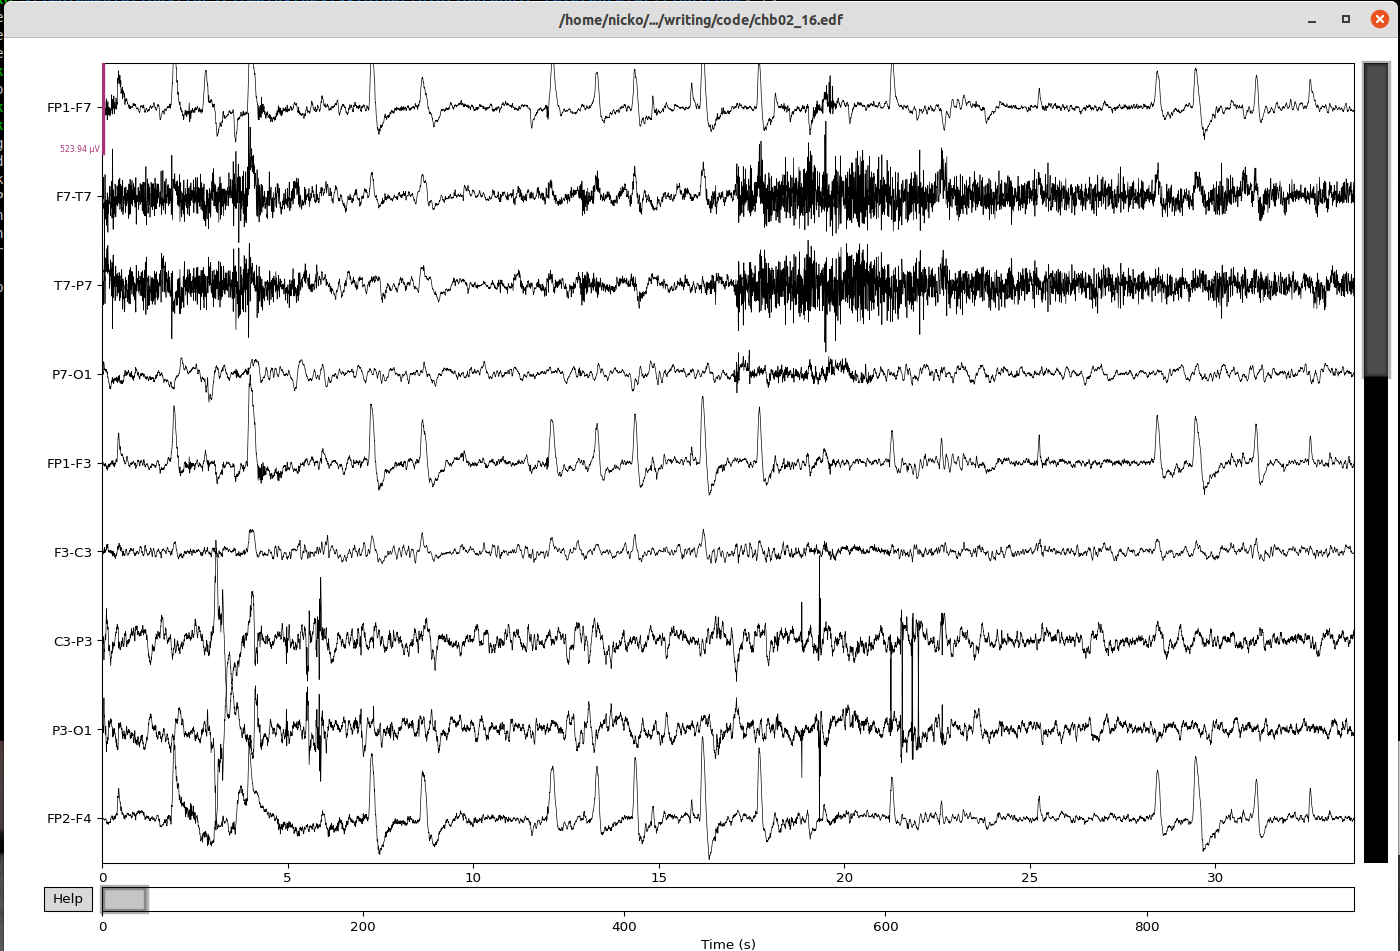
\includegraphics[width=1.1\textwidth]{edf_rec.png}
			    \caption{EEG recording visualized utilizing Python-MNE, for a patient of the dataset.}
			    \label{}
			\end{figure}



		\newpage
		\section{Filtering}

			Electroencephalogram signals in most cases are contaminated by noise 
			and artifacts from physiological (eye blinks, muscle or cardiac activity) 
			and non-physiological sources (powerline interference). 
			In general, artifacts consist of all the non-neural signals 
			that contaminate the recorded EEG data. 
			
			Preprocessing is required in order to increase 
			the quality of the signal(signal-to-noise)
			for boosting further analysis in various application 
			domains like brain-computer interfaces (BCIs) 
			or clinical diagnostics [29-32].
			%\cite{dhanaseivam2023}\cite{jiang2019}\cite{sen2023}\cite{removeArtifactsReview}.
			
			Common preprocessing techniques include:  
			\begin{itemize}  
			    \item \textbf{Filtering} (e.g., Butterworth, Chebyshev) to remove unwanted frequency bands.  
			    \item \textbf{Regression methods} for correcting ocular artifacts using reference channels.  
			    \item \textbf{Blind Source Separation (BSS)} (e.g., ICA, CCA) to decompose and isolate neural activity from artifacts.  
			    \item \textbf{Wavelet/EMD-based methods} for non-stationary artifact removal.  
			\end{itemize}  
			
			Also hybrid approaches (e.g., wavelet-ICA) combine multiple techniques for improved artifact rejection. 
			The choice of method depends on computational constraints, artifact type, 
			and real-time processing needs. 
			Effective preprocessing is a key that ensures reliable feature extraction for later analysis.  

			Among these, wavelet-based methods have have been proposed and used 
			for effecting EEG denoising due to the non stationary nature of brain signals.
			Transient artifacts appearing in EEGs in varying frequency patterns are the reason that 
			traditional linear filtering methods are facing difficulties to handle them 
			without introducing distortions.
			Wavelet transforms on the other hand, decompose the signal 
			into time-frequency representations using scalable, 
			localized basis functions called wavelets, 
			enabling the analysis: the signal is broken down into approximation (low-frequency) 
			and detail (high-frequency) coefficients across decomposition levels. 
			Artifacts, such as ocular blinks or EMG bursts, 
			manifest as sparse, high-amplitude coefficients that can be selectively 
			silenced using thresholds (f.e, hard or soft), 
			followed by reconstruction---thus removing noise while preserving neural transients like epileptic 
			spikes \cite{grobbelaar2022survey}. 

			\subsection{Evaluation metrics for EEG denoising in the CHB-MIT dataset}

			In order to evaluate the performance of 
			different wavelet-based filters for EEG denoising, 
			quantitative metrics have been computed over entire recordings 
			per channel and filter configuration. 
			Metrics used were:

			\begin{itemize}
			    \item \textbf{Signal-to-Noise Ratio (SNR, dB)}: Measures the ratio between the power of the clean 
				    signal and the power of the noise. Higher values indicate better noise suppression 
				    while preserving the structure of the signal.
			    \item \textbf{Root Mean Square Error (RMSE, $\mu$V)}: This metric quantifies 
				    the average deviation between the denoised and reference signals in microvolts. 
					Lower values indicate closer similarity to the original signal.
			    \item \textbf{Normalized RMSE (NRMSE, \%)}: RMSE normalized by the dynamic range of the 
				    reference signal, expressed as a percentage. 
					Lower values represent better performance.
			    \item \textbf{Correlation Coefficient}: Pearson's correlation between the denoised and 
				    reference signals, assessing how similar the two compared waveforms are.
					Values close to $1$ indicate high waveform preservation.
			    \item \textbf{Percent Root-mean-square Difference (PRD, \%)}: Measures the relative distortion 
				    introduced by the denoising process. 
					Lower values indicate less distortion.
			\end{itemize}

			For each one of the filters configuration, metrics were computed 
			channel-wise and then averaged across all channels in order to
			calculate their global performance score. 

			\subsection{Filter Selection Criteria}

			The selection of the optimal filter was based on a multi-criteria ranking strategy, where:
			\begin{enumerate}
			    \item Metrics where \textit{higher} values indicate better performance (\textbf{SNR}, \textbf{Correlation}) were ranked in descending order.
			    \item Metrics where \textit{lower} values indicate better performance (\textbf{RMSE}, \textbf{NRMSE}, \textbf{PRD}) were ranked in ascending order.
			    \item The ranks from all metrics were averaged to obtain an overall performance rank for each filter.
			\end{enumerate}

			The filter with the lowest average rank was considered the best compromise between 
			noise reduction and signal fidelity. According to this 
			evaluation, the \textbf{SYM8, level 4, threshold 0.5, hard thresholding} 
			filter presented the highest overall performance, exhibiting:
			\begin{itemize}
			    \item the highest SNR values,
			    \item one of the lowest RMSE and the lowest NRMSE value,
			    \item the highest correlation coefficient,
			    \item and the lowest PRD.
			\end{itemize}

			This indicates that the chosen filter effectively suppressed noise
			while preserving the morphological features of the EEG signal,
			making it the most suitable choice for subsequent analysis.
			The results of the benchmarking those metrics in 5 EDF 
			recording files which include seizures
			are presented in the following figure.

			\begin{figure}[h]
			    \centering
			    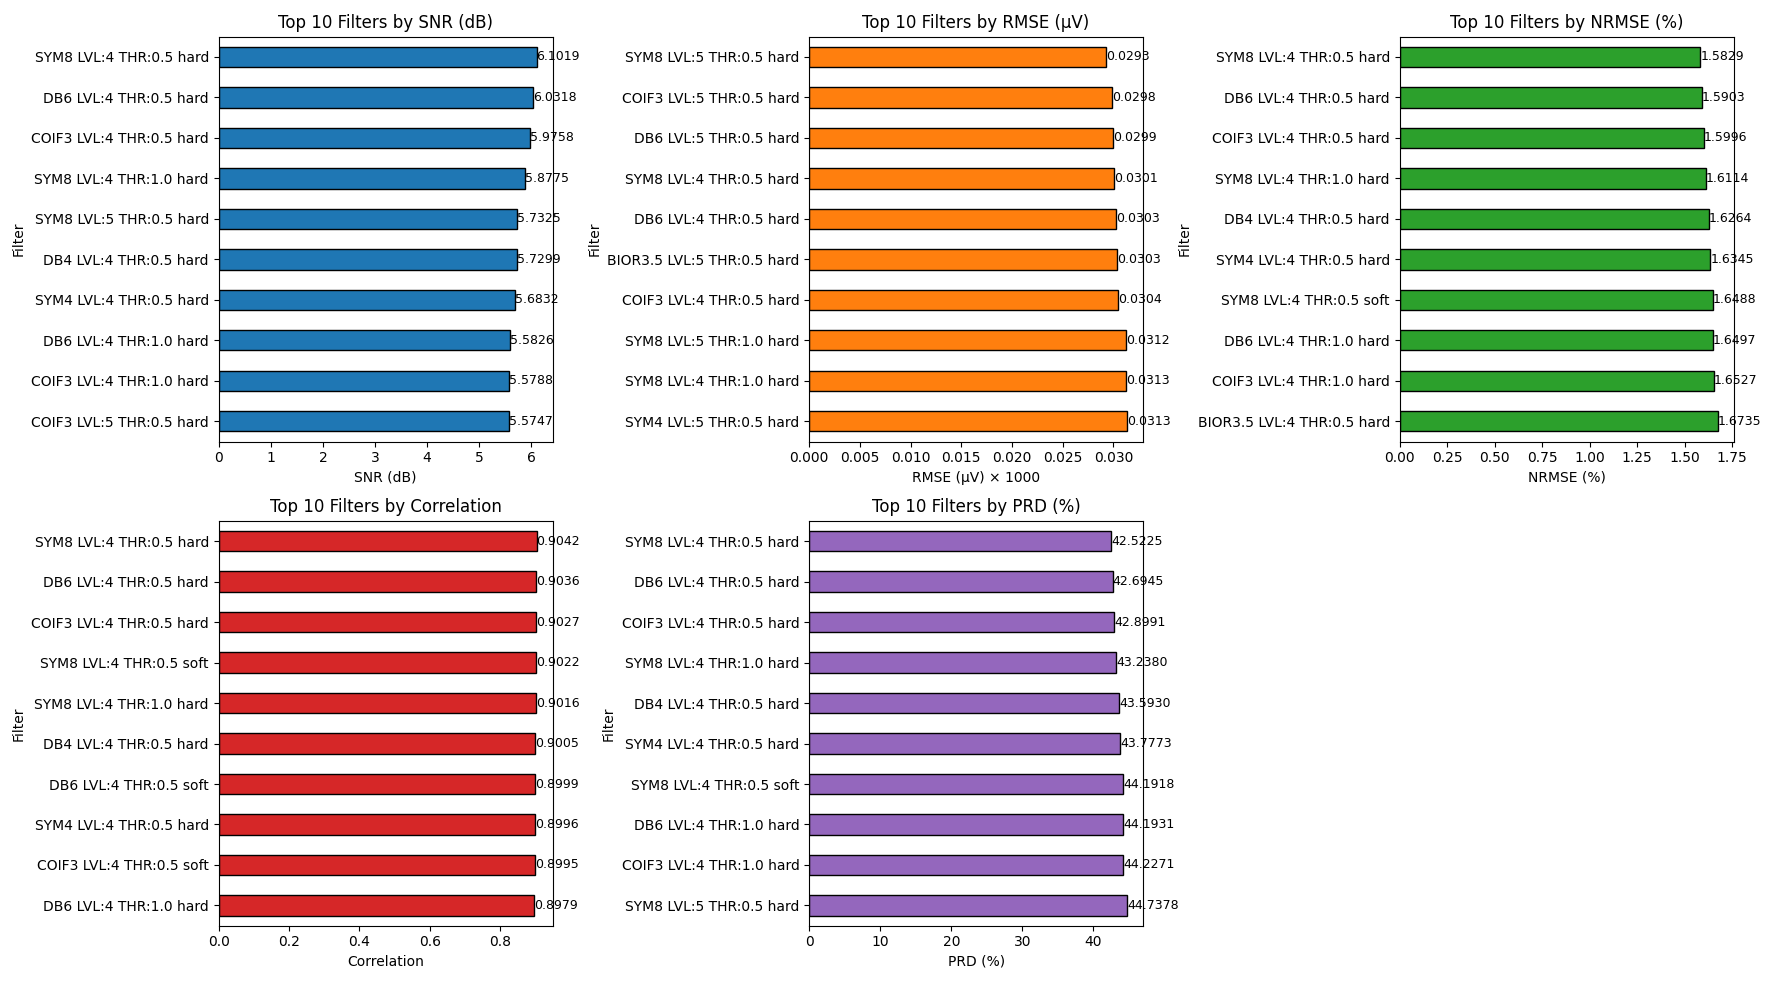
\includegraphics[width=1.1\textwidth]{eeg_metrics_result.png}
			    \caption{The top 10 filter configurations per EEG metric. RMSE values scaled.}
			    \label{}
			\end{figure}

			
			In the following figures we present a visualization using the recording named \textit{chb01\_03.edf}
			comparing the original 10 first EEG channels against the filtered ones with the respective wavelets filters.

			\begin{figure}[H]
			    \centering
			    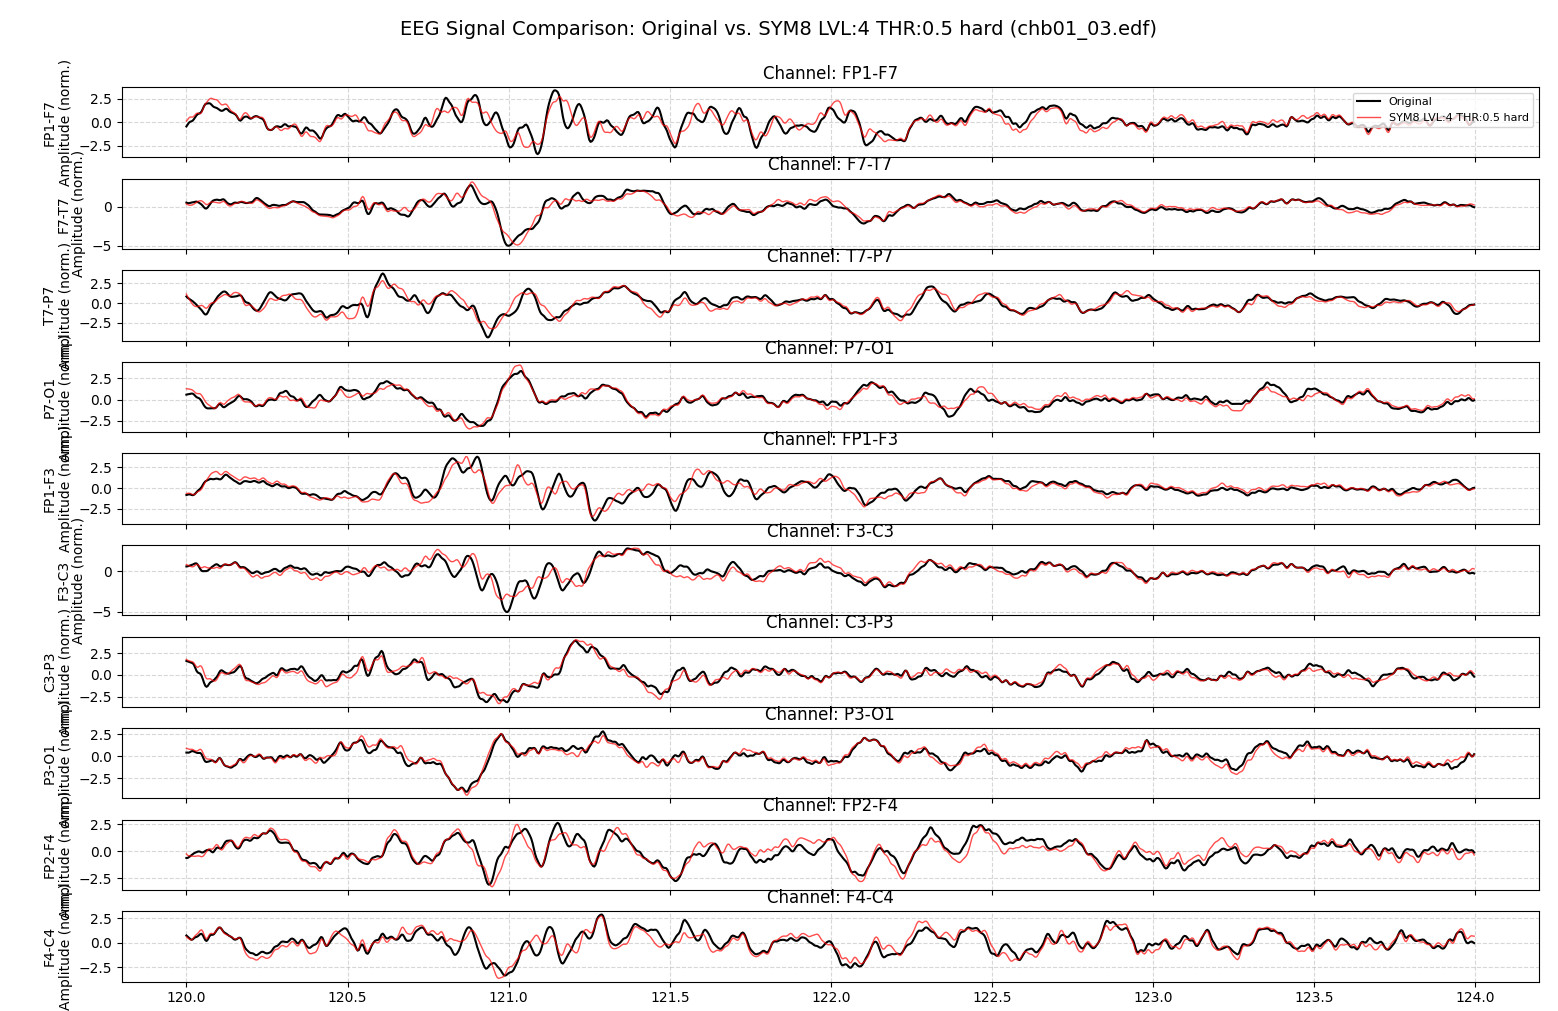
\includegraphics[width=1.2\textwidth]{wav1.png}
			    \caption{}
			    \label{}
			\end{figure}


			\begin{figure}[H]
			    \centering
			    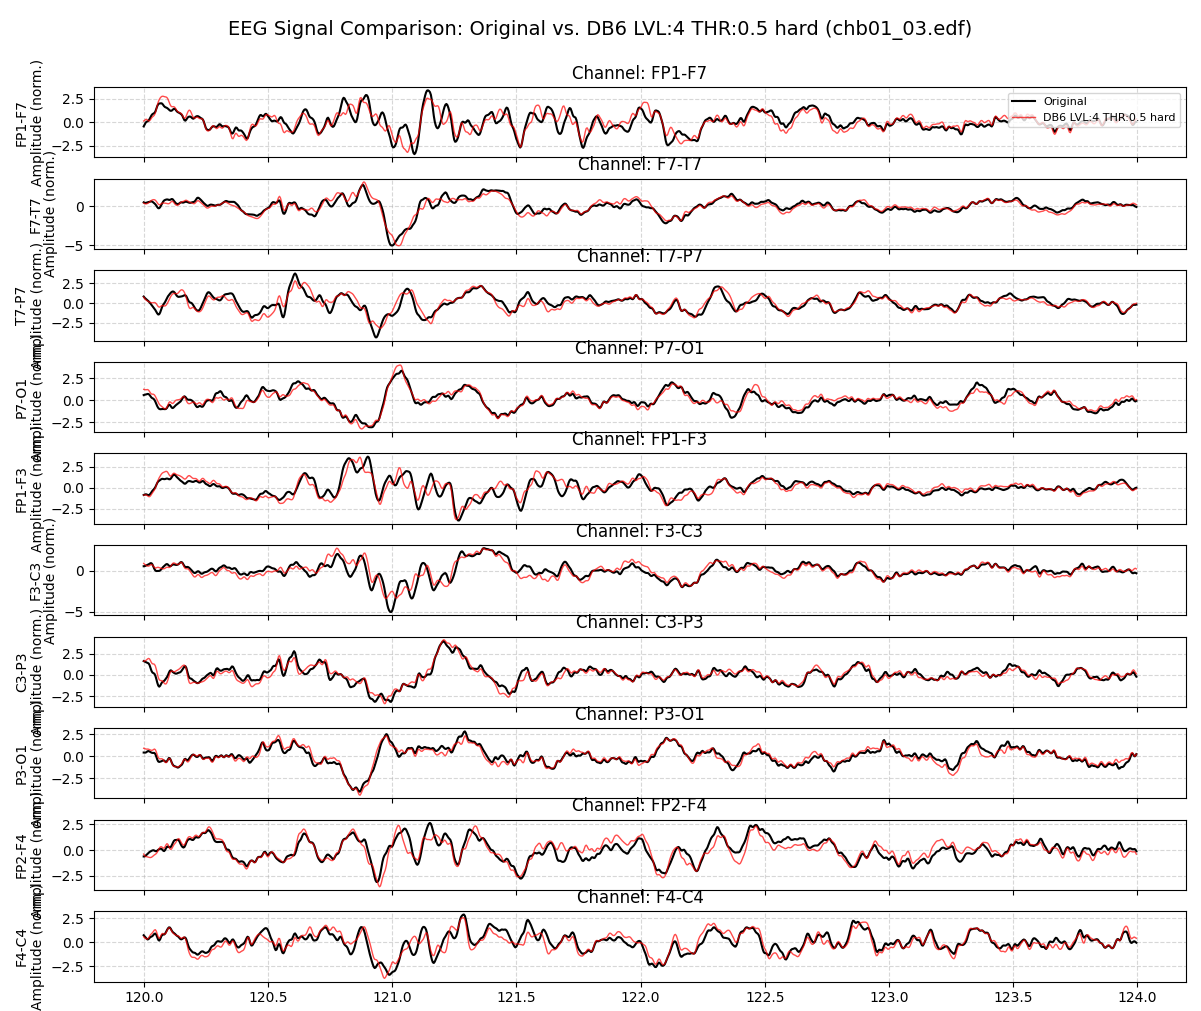
\includegraphics[width=1.2\textwidth]{wav2.png}
			    \caption{}
			    \label{}
			\end{figure}

\begin{comment}
			\begin{figure}[h]
			    \centering
			    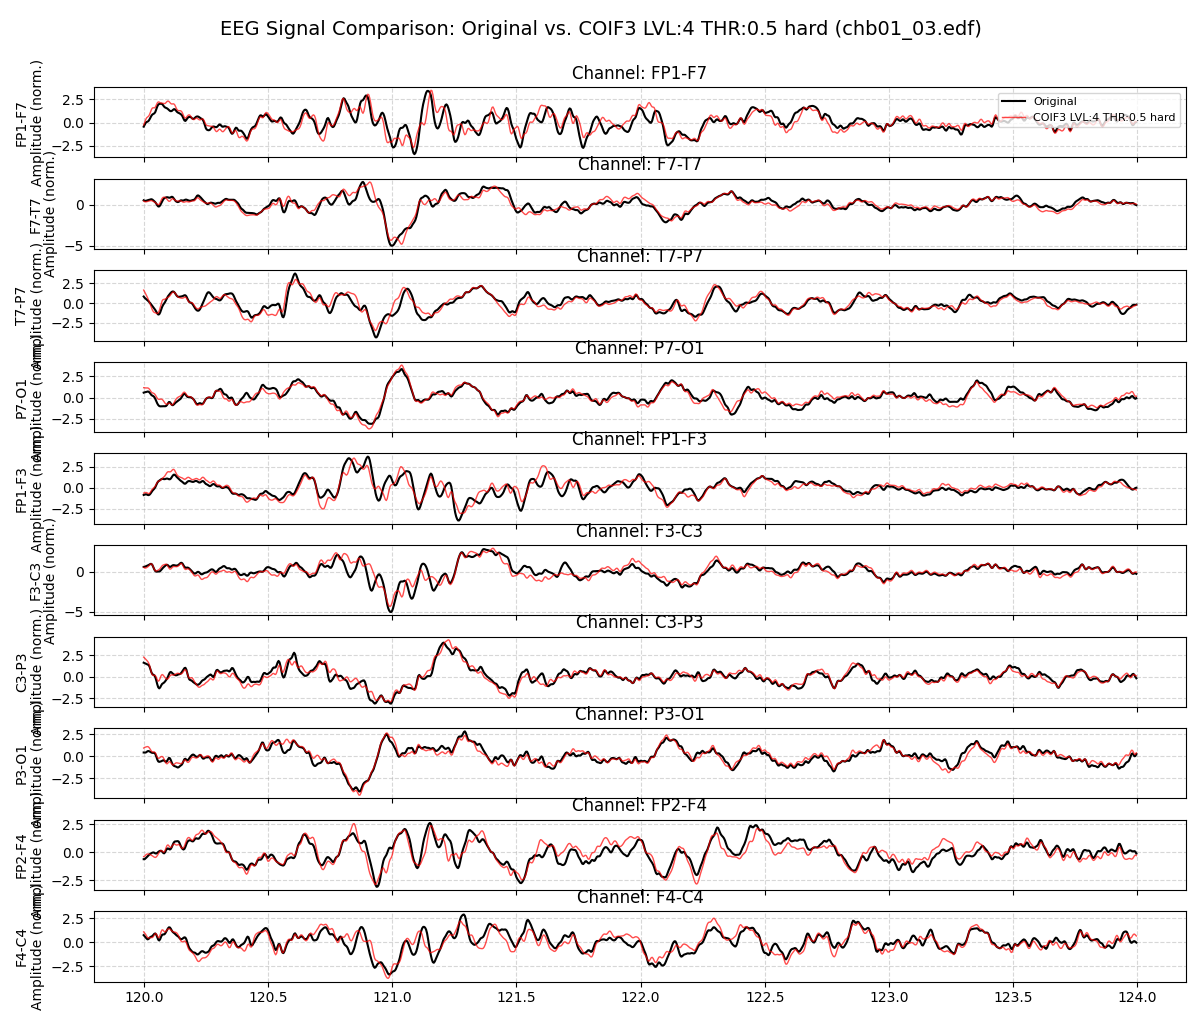
\includegraphics[width=1.2\textwidth]{wav3.png}
			    \caption{}
			    \label{}
			\end{figure}


			\begin{figure}[h]
			    \centering
			    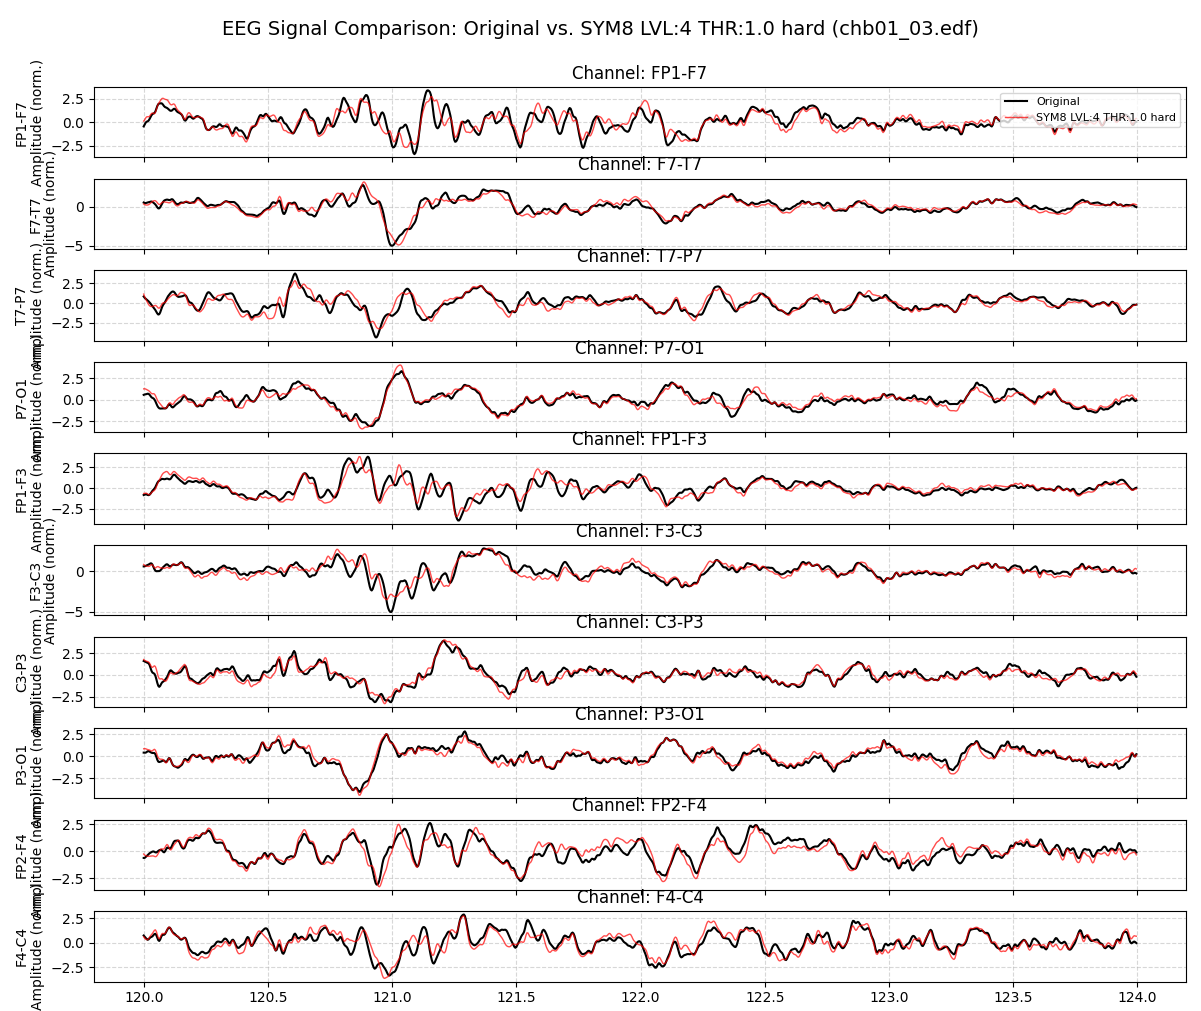
\includegraphics[width=1.2\textwidth]{wav4.png}
			    \caption{}
			    \label{}
			\end{figure}

			\begin{figure}[h]
			    \centering
			    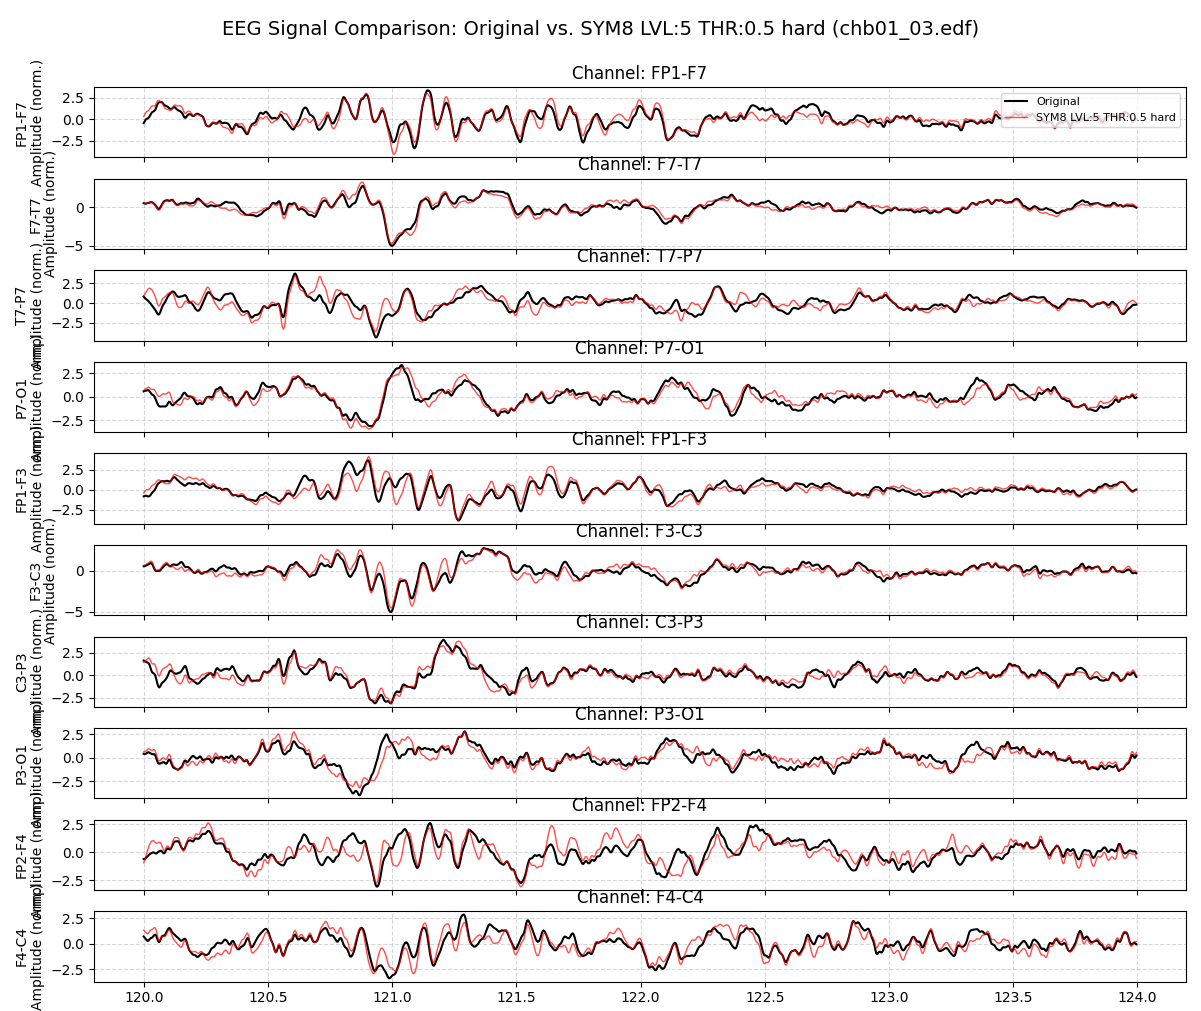
\includegraphics[width=1.2\textwidth]{wav5.png}
			    \caption{}
			    \label{}
			\end{figure}
\end{comment}

	\newpage

		\section{Phase space reconstruction of EEG signals}

			The analysis of nonlinear dynamical systems from experimental time series, requires 
			the reconstruction of the underlying phase space from the scalar measurements of each channel. 
			According to Takens' embedding theorem \cite{takens1981}, a time series $x(t)$ can be embedded 
			in an $m$-dimensional space using time-delay coordinates:

			\begin{equation}
			\vec{y}(t) = \left[x(t), x(t+\tau), x(t+2\tau), \ldots, x(t+(m-1)\tau)\right]
			\end{equation}

			where $m$ is the embedding dimension and $\tau$ is the time delay. The critical challenge lies in determining the appropriate values for these parameters to faithfully reconstruct the system's dynamics without distortion.


	

		\subsection{Determination of Embedding Parameters}
		The reconstruction of the phase space from a single time series 
		\( x(t) \) requires the specification of two parameters: 
		the time delay \( \tau \) and the embedding dimension \( m \). 
		These two parameters determine how the reconstruction will represent
		and how close it will reveal the underlying dynamics without distortion.

			\begin{figure}[H]
				    \centering
				    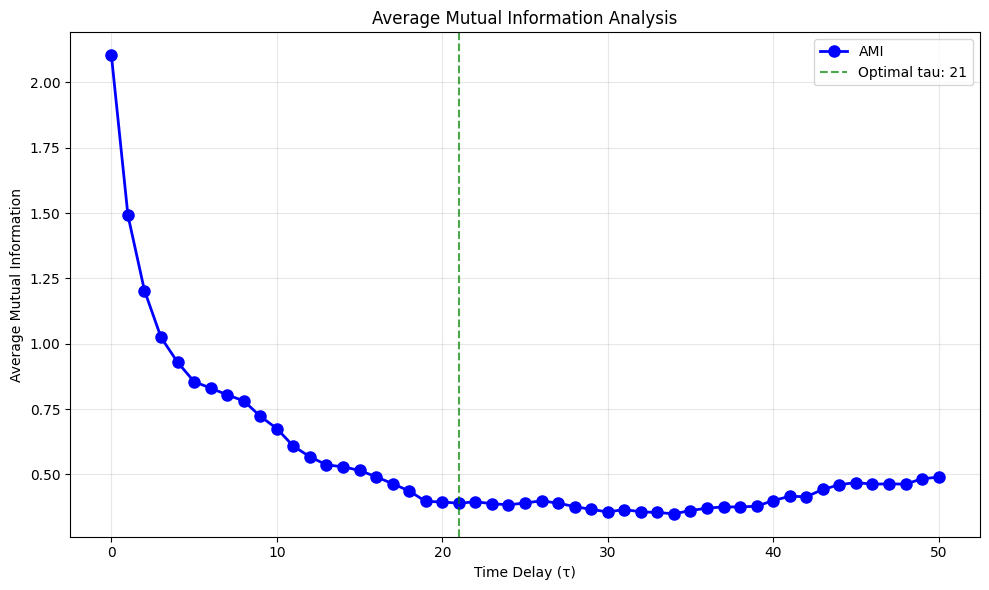
\includegraphics[width=0.8\linewidth]{ami.png}
				    \caption{Calculation of $\tau$ using AMI for a sample EEG channel. The first minimum of the AMI function (green dashed line) is chosen to become the optimal $\tau$ to ensure independence between delay coordinates.}
				    \label{fig:ami_plot}
			\end{figure}



		\subsubsection{Calculation of time delay \( \tau \) utilizing mutual information}
			The time delay \( \tau \) can be estimated by applying the 
			\textit{Average Mutual Information} (AMI) method, a concept which was first introduced 
			by Fraser and Swinney~\cite{fraser1986}. 
			In contrast to linear autocorrelation, 
			mutual information has the ability to capture both linear and nonlinear dependencies among
			the original time series \( x(t) \) and its delayed version \( x(t + \tau) \).

			The mutual information \( I(\tau) \) between \( x(t) \) and \( x(t + \tau) \) is defined as:
			\[
			I(\tau) = \sum_{x(t),\, x(t+\tau)} P(x(t), x(t+\tau)) \, \log_2 \left( \frac{P(x(t), x(t+\tau))}{P(x(t)) \, P(x(t+\tau))} \right)
			\]
			where \( P(\cdot) \) denotes probability.

			The optimal time delay \( \tau \) is chosen as the value at which 
			\( I(\tau) \) reaches its \textit{first minimum}. 
			This value indicates a good compromise 
			between independence (too small \( \tau \)) and irrelevance (too large \( \tau \)) 
			of the coordinates in the embedding vector.
				

		


			\subsubsection{Estimating embedding dimension \( m \) using false nearest neighbors approach}

			When the embedding dimension $m$ is too small, 
			the phase space becomes \emph{projected} rather than 
			properly \emph{embedded}. 
			This projection can create artificial neighborhoods where points appear to be close due to 
			geometrical constraints of the space rather than their actual dynamical similarity. 
			These are named as \emph{false nearest neighbors} \cite{kennel1992}.


				\begin{figure}[h!]
				    \centering
				    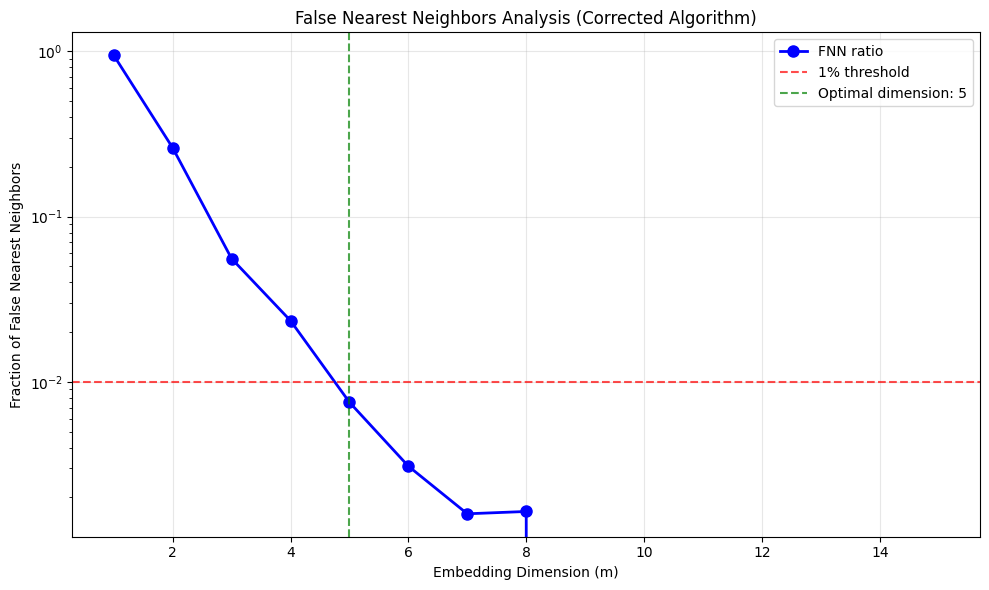
\includegraphics[width=0.8\linewidth]{fnn_estim.png}
				    \caption{Calculation of the embedding dimension using the FNN scheme.}
				    \label{fig:fnn_plot}
				\end{figure}


			\begin{figure}[h]
			\centering
			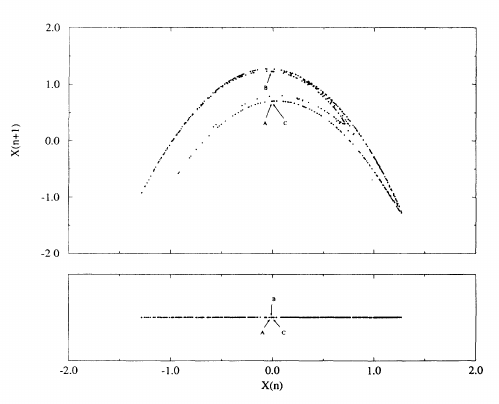
\includegraphics[width=0.8\textwidth]{fnn_schematic.png}
			\caption{Schematic illustration of false neighbors. In insufficient embedding dimension (down), points A and B appear neighbors due to projection. When proper embedding is employed(up), their true separation is revealed.}
			\label{fig:fnn_schematic}
			\end{figure}

			Mathematically, two points $\vec{y}_i$ and $\vec{y}_j$ are false neighbors if their distance increases significantly when embedded in higher dimension:

			\begin{equation}
			\frac{\|\vec{y}_i^{(m+1)} - \vec{y}_j^{(m+1)}\|}{\|\vec{y}_i^{(m)} - \vec{y}_j^{(m)}\|} > R_{\text{tol}}
			\end{equation}

			where $R_{\text{tol}}$ is a tolerance threshold (typically 10--15).

			The False Nearest Neighbors(FNN) method \cite{kennel1992} 
			provides a systematic approach in order to determine the 
			minimal sufficient embedding dimension. The method's steps are:

			\begin{enumerate}
			\item For each point in dimension $m$, identify its nearest neighbor.
			\item Embed the data in dimension $m+1$.
			\item Calculation the relative distance increase between each point and its former neighbor.
			\item If the increase exceeds predetermined thresholds, the neighbor point is classified as a false neighbor
			\item The optimal $m$ is the smallest dimension where the fraction of 
				false neighbors drops below an acceptable level (typically 1--5\%)
			\end{enumerate}

			Both relative and absolute criteria are included in the algorithm:

			\begin{align}
			\text{Relative:} &\quad \frac{\|\vec{y}_i^{(m+1)} - \vec{y}_j^{(m+1)}\|}{\|\vec{y}_i^{(m)} - \vec{y}_j^{(m)}\|} > R_{\text{tol}} \\
			\text{Absolute:} &\quad \|\vec{y}_i^{(m+1)} - \vec{y}_j^{(m+1)}\| > A_{\text{tol}} \cdot \sigma_x
			\end{align}

			where $\sigma_x$ is the standard deviation of the time series.
			



			When optimal parameters $\tau$ and $m$ have been determined for a given signal, 
			the phase space can be reconstructed according to Takens' theorem. This reconstruction provides the
			geometric picture of the underlying dynamics.

			Figure \ref{fig:phase_space_3d} presents the reconstructed phase space for a normal EEG segment from channel 'Fp1-F7' from CHB-MIT 's chb24\_01.edf data.

				\begin{figure}[h!]
				    \centering
				    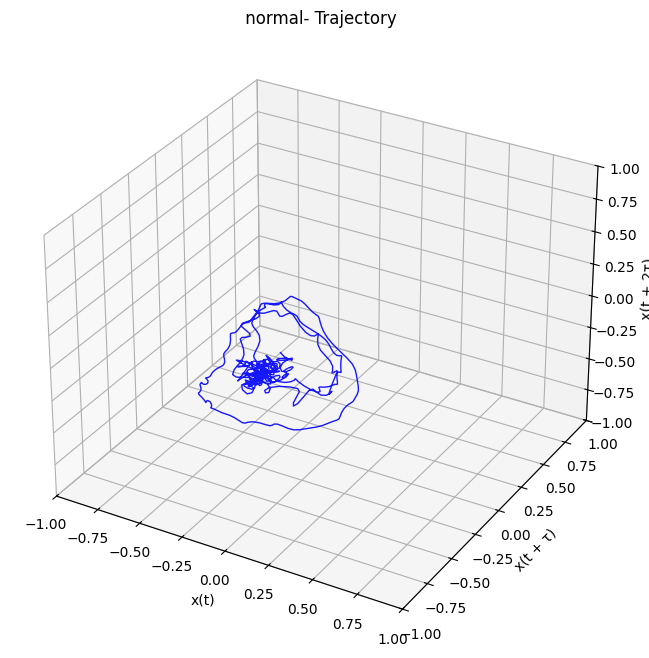
\includegraphics[width=0.7\linewidth]{phase_space_3d.png} % Assuming you make a 2-panel figure
				    \caption{3D phase space reconstruction for a 3-second EEG segment's channel.}
				    \label{fig:phase_space_3d}
				\end{figure}



			%%% NOTE: commented maybe not to write? 
			%Applying FNN to EEG data is particularly 
			%important for several reasons. EEG signals exhibit 
			%nonstationary characteristics, making fixed embedding parameters 
			%suboptimal and contain measurement noise and artifacts 
			%that can distort phase space reconstruction. 
			%In addition the optimal embedding may vary across subjects, 
			%brain states, and recording conditions and FNN provides a data-driven approach that adapts to individual recordings.




					
	\newpage
						% ===== Page X =====
				\section{Recurrence Quantification Analysis (RQA)}

				Having reconstructed the phase space trajectory of the EEG signals, 
				the next step is to analyze its dynamical properties. 
				Recurrence Quantification Analysis is a powerful nonlinear method that 
				provides precisely this functionality by quantifying the number and duration 
				of recurrences of a dynamical system to its previous states \cite{theoryReviewRQA}. 
				The core of this quantification process is the \emph{Recurrence Plot (RP)}, 
				a visualization which denotes the times at which the phase space 
				trajectory revisits approximately the same area.
				In most non trivial cases, a phase space  does not have a dimension (two or three)
				which allows a direct visualization, so for higher dimensional phase spaces 
				the only solution is a projection into a two or three dimensional space. 
				However, RP enables the examination of a higher-dimensional phase space trajectory 
				via its two-dimensional representation of its recurrences.

				\subsection{The Recurrence Plot (RP)}

				RP is a symmetric, two-dimensional matrix that visualizes the recurrences of states.
				For a reconstructed trajectory \(\vec{y}(t)\) of length \(N\), 
				the recurrence matrix \(\mathbf{R}\) is defined as:

				\begin{equation}
				R_{i,j} = \Theta(\varepsilon - \|\vec{y}(i) - \vec{y}(j)\|), \quad i,j = 1, \ldots, N
				\end{equation}

				where:
				\begin{itemize}
				    \item \(\Theta(\cdot)\) is the Heaviside step function (\(\Theta(x)=0\) if \(x<0\), and \(\Theta(x)=1\) otherwise),
				    \item \(\varepsilon\) is a predefined distance threshold (radius),
				    \item \(\|\cdot\|\) is a norm.
				\end{itemize}
	
				By interpreting the RP, several metrics can be extracted for further analysis.
				
				\subsection{Key RQA Metrics and Their Interpretation}
					\label{subsec:rqa_metrics}

					RQA provides a set of metrics that can quantify the 
					number and the duration of the recurrences of a dynamical system.
					These metrics are categorized by those which are based on diagonal structures, 
					which relate to the predictability and deterministic nature of the system, 
					and those that are based on vertical structures, which can capture laminar 
					states or chaos-chaos transitions.

					The definitions of the core RQA metrics, as implemented in tools like the utilized \texttt{PyRQA}, 
					are as follows \cite{marwan_website}:

					\begin{description}

					\item[Recurrence Rate (\textbf{RR})]
					The recurrence rate is the simplest measure, defined as the density of recurrence points in the RP. It corresponds to the probability that a state recurs and is analogous to the correlation sum.
					\[
					RR = \frac{1}{N^2} \sum_{i,j=1}^{N} R_{i,j}
					\]

					\item[Determinism (\textbf{DET})]
					Determinism quantifies the percentage of recurrence points that form diagonal lines. Diagonal lines are a signature of deterministic dynamics, where segments of the trajectory run in parallel for some time. A higher DET indicates a more predictable, deterministic system.
					\[
					DET = \frac{\sum_{l=l_{\text{min}}}^{N} l \, P(l)}{\sum_{l=1}^{N} l \, P(l)}
					\]
					where \( P(l) \) is the histogram of diagonal line lengths \( l \), and \( l_{\text{min}} \) is the minimum line length (typically 2).

					\item[Laminarity (\textbf{LAM})]
					Laminarity measures the percentage of recurrence points that form vertical lines. Vertical lines indicate states that do not change or change very slowly for a period (laminar states). It can detect chaos-chaos transitions or intermittency.
					\[
					LAM = \frac{\sum_{v=v_{\text{min}}}^{N} v \, P(v)}{\sum_{v=1}^{N} v \, P(v)}
					\]
					where \( P(v) \) is the histogram of vertical line lengths \( v \), and \( v_{\text{min}} \) is the minimum line length.

					\item[Ratio (\textbf{RATIO})]
					The ratio is a measure of complexity, calculated as the ratio between DET and RR. It can be sensitive to transitions between order and chaos.
					\[
					RATIO = \frac{N^2 \sum_{l=l_{\text{min}}}^{N} l \, P(l)}{\left( \sum_{l=1}^{N} l \, P(l) \right)^2}
					\]

					\item[Average Diagonal Line Length (\textbf{L})]
					This metric represents the average time that two segments of the trajectory remain close, providing an estimate of the mean prediction time.
					\[
					L = \frac{\sum_{l=l_{\text{min}}}^{N} l \, P(l)}{\sum_{l=l_{\text{min}}}^{N} P(l)}
					\]

					\item[Trapping Time (\textbf{TT})]
					Trapping time is the average length of vertical lines, quantifying the mean time the system remains trapped in a specific state (laminarity in time).
					\[
					TT = \frac{\sum_{v=v_{\text{min}}}^{N} v \, P(v)}{\sum_{v=v_{\text{min}}}^{N} P(v)}
					\]

					\item[Longest Diagonal Line (\textbf{L$_{\text{max}}$})]
					The length of the longest diagonal line in the RP is related to the Lyapunov exponent of the system. A shorter \( L_{\text{max}} \) suggests a faster divergence of trajectories, which is a hallmark of chaos.
					\[
					L_{\text{max}} = \max(\{l_i \; | \; i=1,\ldots,N_l\})
					\]

					\item[Divergence (\textbf{DIV})]
					Divergence is the inverse of \( L_{\text{max}} \). It is related to the Kolmogorov-Sinai entropy and the sum of the positive Lyapunov exponents, providing a measure of how quickly nearby trajectories diverge.
					\[
					DIV = \frac{1}{L_{\text{max}}}
					\]

					\item[Longest Vertical Line (\textbf{V$_{\text{max}}$})]
					The length of the longest vertical line is another indicator of the system's laminar behavior.
					\[
					V_{\text{max}} = \max(\{v_i \; | \; i=1,\ldots,N_v\})
					\]

					\item[Entropy (\textbf{ENTR})]
					The Shannon entropy of the probability distribution \( p(l) \) of the diagonal line lengths. It reflects the complexity of the deterministic structure in the system. A higher ENTR indicates a more complex and less periodic dynamics.
					\[
					ENTR = - \sum_{l=l_{\text{min}}}^{N} p(l) \ln p(l), \quad \text{where } p(l) = \frac{P(l)}{\sum_{l=l_{\text{min}}}^{N} P(l)}
					\]

					\item[Trend (\textbf{TREND})]
					Trend quantifies the paling of the RP towards its edges, which can be caused by non-stationarity in the data (e.g., a slow drift in the mean of the signal). It is calculated as the slope of the linear regression of the local recurrence rate \( RR_i \) over the distance from the main diagonal.
					\[
					TREND = \frac{\sum_{i=1}^{\tilde{N}} (i - \tilde{N}/2)(RR_i - \langle RR_i \rangle)}{\sum_{i=1}^{\tilde{N}} (i - \tilde{N}/2)^2}
					\]
					where \( \tilde{N} \) is the number of diagonals parallel to the Line of Identity (LOI) that are considered, and \( RR_i \) is the recurrence rate in the \( i \)-th diagonal.

					\end{description}

					These metrics, when applied to EEG signals, allow for the characterization of the brain's dynamic states. For instance, in epilepsy detection, seizures (ictal states) often exhibit higher determinism (DET) and laminarity (LAM) compared to the more stochastic and complex inter-ictal states, making RQA a powerful tool for identifying pathological patterns.	


				


				\subsection{From RQA to Cross-Recurrence Quantification Analysis (CRQA)}
					\label{subsec:crqa_theory}

					While Recurrence Quantification Analysis (RQA) is powerful for analyzing the dynamics of a single system, many real-world phenomena, including brain activity, involve the interaction between multiple subsystems. Cross-Recurrence Quantification Analysis (CRQA) extends the concepts of RQA to analyze the coupling, synchronization, and similarity in the dynamics between two different systems \cite{marwan2007}.

					\subsubsection{The Cross-Recurrence Plot (CRP)}

					The foundation of CRQA is the Cross-Recurrence Plot (CRP). For two reconstructed phase space trajectories \( \vec{x}(i) \) from system \( X \) and \( \vec{y}(j) \) from system \( Y \), both of length \( N \), the cross-recurrence matrix is defined as:

					\begin{equation}
					CR_{i,j} = \Theta(\varepsilon - \|\vec{x}(i) - \vec{y}(j)\|), \quad i,j = 1, \ldots, N
					\end{equation}

					Unlike the standard RP, which is symmetric about the main diagonal (Line of Identity, LOI), the CRP is generally \emph{not symmetric}. This asymmetry can reveal directional relationships or leader-follower dynamics between the two systems.

					\subsubsection{Interpretation of CRQA Metrics}

					The same quantitative measures defined for RQA (Section~\ref{subsec:rqa_metrics}) can be applied to the CRP, but their interpretation shifts from describing \emph{self-similarity} to describing \emph{coupling} and \emph{interaction}:

					\begin{itemize}
					    \item \textbf{Cross-Recurrence Rate (CRR)}: The probability that the state of system \( X \) at time \( i \) is close to the state of system \( Y \) at time \( j \). A high CRR indicates overall similar states between the two systems.
					    
					    \item \textbf{Cross-Determinism (CDET)}: The percentage of recurrent points in the CRP that form diagonal lines. Diagonal lines occur when the two systems follow a similar path in phase space for some time. \textbf{This is a crucial metric for epilepsy detection}, as it quantifies the transient synchronization between different brain regions. A seizure often manifests as increased CDET between channels in the epileptogenic zone.
					    
					    \item \textbf{Cross-Laminarity (CLAM)}: Measures the laminarity between the two systems, indicating when one system gets trapped in a state while the other changes.
					    
					    \item \textbf{Average Diagonal Line Length (L)} in the CRP estimates the mean time that the two systems remain synchronized or follow a similar trajectory.
					\end{itemize}

					\subsubsection{Why CRQA for Multi-Channel EEG?}

					Applying CRQA to pairs of EEG channels is particularly well-suited for epilepsy detection for several reasons:

					\begin{itemize}
					    \item \textbf{Synchronization Detection}: Epileptic seizures are characterized by abnormal, excessive synchronization of neuronal populations. CRQA directly quantifies this synchronization in the phase space.
					    \item \textbf{Nonlinear and Non-stationary}: CRQA does not assume linearity or stationarity, making it robust for analyzing the complex, transient dynamics of EEG signals.
					    \item \textbf{Directional Insights}: While not explored in all analyses, the potential asymmetry of the CRP can, in principle, help identify the propagation path of a seizure.
					    \item \textbf{Focus on Interaction}: It moves beyond analyzing individual channels in isolation to directly measure the dynamic interplay between different brain regions, which is often where the pathology lies.
					\end{itemize}

					In this thesis, CRQA is employed to compute a set of features (Table~\ref{tab:pyrqa_metrics}) for all unique pairs of EEG channels. These features capture the complex synchronization patterns that distinguish pre-ictal, ictal, and inter-ictal states, forming the basis for the subsequent machine learning classification.





	\newpage

					
				\section{Methodology}
				\label{sec:methodology}

				In this section the methodology for processing EEG data is described in order to perform CRQA to analyze epileptic and non-epileptic brain activity. 
				The approach consists of different parts such as loading and segmenting EEG recordings, 
				extracting non-overlapping time windows, selecting the embedding parameters and computing CRQA features for channel pairs. 
				The methodology is implemented in Python using libraries such as \texttt{numpy}, \texttt{torch}, \texttt{pyopencl}, and \texttt{pyrqa} \cite{pyrqacitation}.

				\subsection{Data preprocessing and windowing}
				\label{subsec:data_preprocessing}

				Prior filtererd EEG recordings are stored in NumPy array format (\texttt{.npy}), 
				accompanied by metadata specifying the sampling frequency (\(f_s\)) and channel information (22 channels with their respective labels as \texttt{FP1-F7}, \texttt{F7-T7}, ..., \texttt{FT10-T8}). 
				The time axis is computed as \(t = \frac{n}{f_s}\), where \(n\) is the sample index and \(f_s\) is the sampling frequency in Hertz (Hz).

				Each EEG channel is segmented into continuous regions based on predefined boundaries from CHB-MIT dataset \cite{chbmitDataset} annotations, distinguishing epileptic from non-epileptic segments. 
				Then, each segment is further divided into non-overlapping time windows of fixed size (512 samples, equivalent to 2 seconds at 256 Hz). 
				For each segment, the number of windows is calculated by performing integer division of the segment length by the window size and discarding any incomplete windows. 
				Each window is associated with a segment index, window index within the segment, start and end sample indices, and a label (1 for epileptic, 0 for non-epileptic).

				\subsection{Embedding parameters selection}
				\label{subsec:embedding_parameters}
				
				The embedding dimension \texttt{m} and time delay $\tau$ were set to 3 and 1, respectively, 
				following common practice in EEG analysis. This choice was also motivated by known limitations that the FNN algorithm experiences 
				when applied to noisy and autocorrelated signals, such as EEG. 
				For instance, \cite{FredkinRiceFNN} have shown that FNN can falsely indicate low-dimensional determinism in 
				autocorrelated stochastic processes, while \cite{RhodesMorariFNN} showed that the effects of noise can actually
				lead in overestimation of the embedding dimension. 
				In order to mitigate these effects and keep a consist methodology across a 
				large dataset, the presented methodology adopts fixed values for the embedding parameters rather than optimizing them
				per recording or window.
				The decision to use constant values is influenced by applied precedents in the EEG literature. 
				McSharry et al.\cite{mcsharry} have applied with success fixed embedding parameters in their multi-channel scalp EEG seizure research, 
				arguing that nonlinear methods must justify their complexity over simpler linear benchmarks. 
				In our case, fixed parameters ensure consistency across the large CHB-MIT dataset and help avoid overfitting to local dynamics that may not generalize.
				
				\subsection{Threshold selection}
				Radius fraction R is utilized for determination of the percentage of mean diameter of the 
				reconstructed phase space where a recurrence can occur.
				In order to estimate and standardize R,
				an exploration of its effect on CRPs and RR/DET metrics is performed. 
				By keeping constant $\tau = 1$ and \textbf{\textit{m}} = 3
				CRPs are generated by selecting random patients and random recording windows of the dataset,
				while computing the mean channel-wise recurrence rate and mean channel-wise determinism 
				from the 22x22 CRPs features.

				Results of RR and DET are presented in the following table.
				The different explored values for radius fraction are set to be 
				{ 0.1, 0.15, 0.20 and 0.30} for this experiment.
								
				\begin{table}[h!]
				\centering
				\caption{Comparison of RR and DET values for different radius (R) values}
				\begin{tabular}{l S[table-format=1.2] S[table-format=2.2] S[table-format=2.2] l}
				\toprule
				\textbf{Recording} & \textbf{R} & \textbf{RR (\%)} & \textbf{DET (\%)} & \textbf{Window} \\
				\midrule
				patient\_24 & 0.10 & 9 & 77.36 & Normal \\
				patient\_24 & 0.15 & 16.7 & 85.3 & Normal \\
				patient\_24 & 0.20 & 23.8 & 89 & Normal \\
				patient\_24 & 0.30 & 36.4 & 93.25 & Normal \\
				patient\_24 & 0.10 & 16.35 & 97.6 & Epileptic \\
				patient\_24 & 0.15 & 26 & 99 & Epileptic \\
				patient\_24 & 0.20 & 35.16 & 99.44 & Epileptic \\
				patient\_24 & 0.30 & 51.9 & 99.74 & Epileptic \\
				\midrule
				patient\_10 & 0.10 & 10.6 & 83.5 & Normal \\
				patient\_10 & 0.15 & 16.54 & 86.8 & Normal \\
				patient\_10 & 0.20 & 22.13 & 88.97 & Normal \\
				patient\_10 & 0.30 & 32.5 & 92.87 & Normal \\
				patient\_10 & 0.10 & 14.94 & 93.6 & Epileptic \\
				patient\_10 & 0.15 & 22.9 & 95.7 & Epileptic \\
				patient\_10 & 0.20 & 30.3 & 96.41 & Epileptic \\
				patient\_10 & 0.30 & 43.59 & 97.16 & Epileptic \\
				\midrule
				patient\_8 & 0.10 & 7.08 & 59.26 & Normal \\
				patient\_8 & 0.15 & 11.82 & 65,12 & Normal \\
				patient\_8 & 0.20 & 16.33 & 67.59 & Normal \\
				patient\_8 & 0.30 & 24.76 & 71.73 & Normal \\
				patient\_8 & 0.10 & 16.4 & 98.3 & Epileptic \\
				patient\_8 & 0.15 & 25 & 99.46 & Epileptic \\
				patient\_8 & 0.20 & 33.1 & 99.60 & Epileptic \\
				patient\_8 & 0.30 & 47.71 & 99.76 & Epileptic \\
				\midrule
				patient\_1 & 0.10 & 18.31 & 96.02 & Normal \\
				patient\_1 & 0.15 & 27.83 & 97.70 & Normal \\
				patient\_1 & 0.20 & 36.61 & 97.89 & Normal \\
				patient\_1 & 0.30 & 52.08 & 98.89 & Normal \\
				patient\_1 & 0.10 & 20.89 & 96.11 & Epileptic \\
				patient\_1 & 0.15 & 33.93 & 98.46 & Epileptic \\
				patient\_1 & 0.20 & 45.61 & 99.22 & Epileptic \\
				patient\_1 & 0.30 & 64.64 & 99.68 & Epileptic \\

				\bottomrule
				\end{tabular}
				\end{table}
				
				As it can be observed, both RR and DET increase while the radius fraction $R$ increases
				for all patients/windows combinations, since by having a larger radius there are more points to be considered as recurrent in the phase space.
				Epileptic windows present consistently higher RR and DET values when compared with normal windows at the same $R$ and same patients.
				It should be noted that there is inter-patient variability also, 
				suggesting that optimal radius selection may benefit from patient-specific tuning.
				Additionally, DET values in epileptic windows approach saturation near 100\% as $R$ increases, a fact that suggests 
				having a moderate radius fraction (e.g., $R = 0.15$--$0.20$) could provide a 
				better balance between sensitivity and specificity in CRP analysis for the determinism metric.


				\begin{figure}[htbp]
				    \centering
				    \begin{subfigure}[t]{0.45\textwidth}
					\centering
					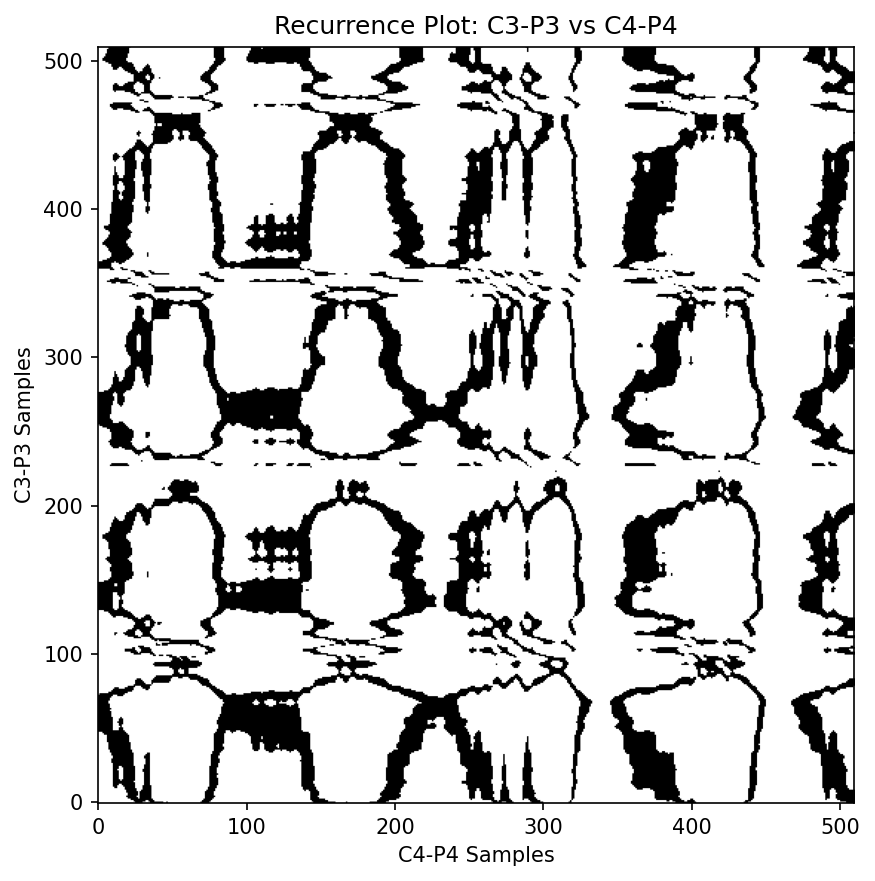
\includegraphics[width=\textwidth]{rr_compare/r01_epil.png}
					\caption{radius fraction = 0.1}
					\label{subfig:rp1}
				    \end{subfigure}
				    \hfill % Adds horizontal space between subfigures
				    \begin{subfigure}[t]{0.45\textwidth}
					\centering
					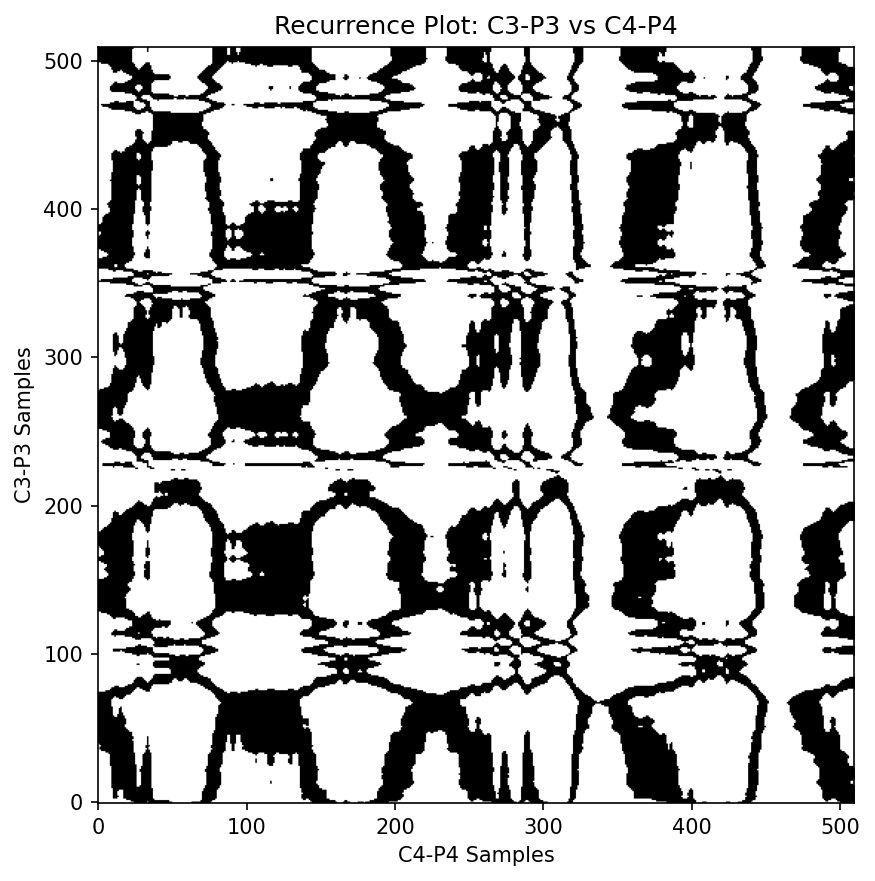
\includegraphics[width=\textwidth]{rr_compare/r015_epil.png}
					\caption{radius fraction = 0.15}
					\label{subfig:rp2}
				    \end{subfigure}

				    \vspace{0.5cm} % Adds vertical space between rows

				    \begin{subfigure}[t]{0.45\textwidth}
					\centering
					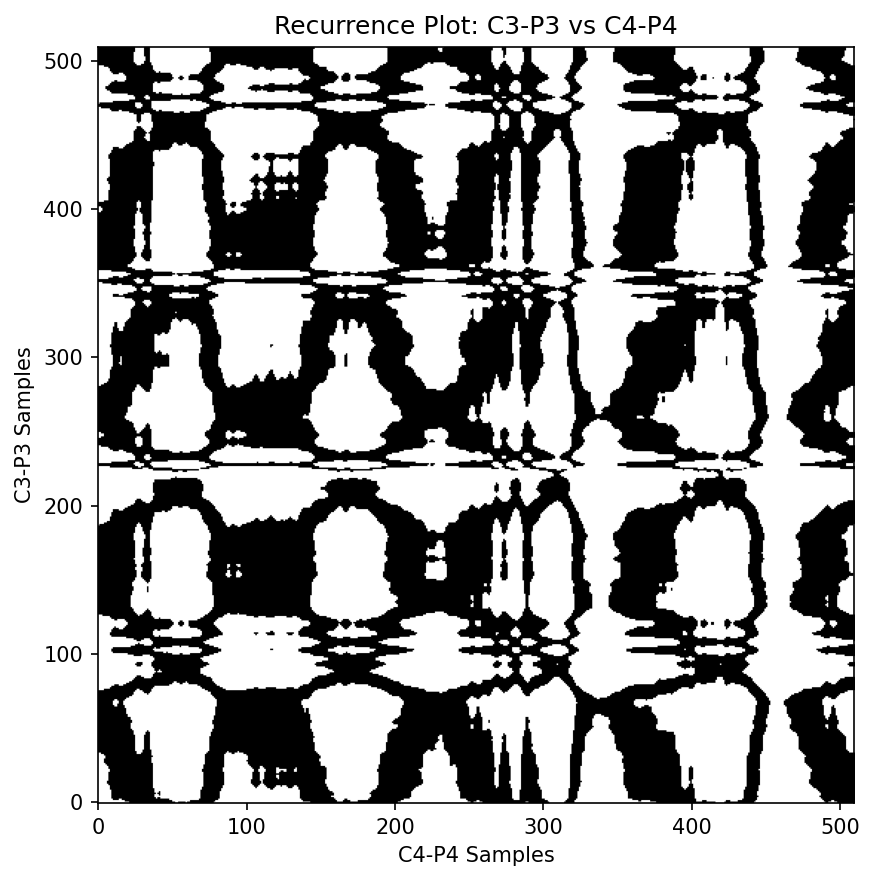
\includegraphics[width=\textwidth]{rr_compare/r02_epil.png}
					\caption{radius fraction = 0.2}
					\label{subfig:rp3}
				    \end{subfigure}
				    \hfill
				    \begin{subfigure}[t]{0.45\textwidth}
					\centering
					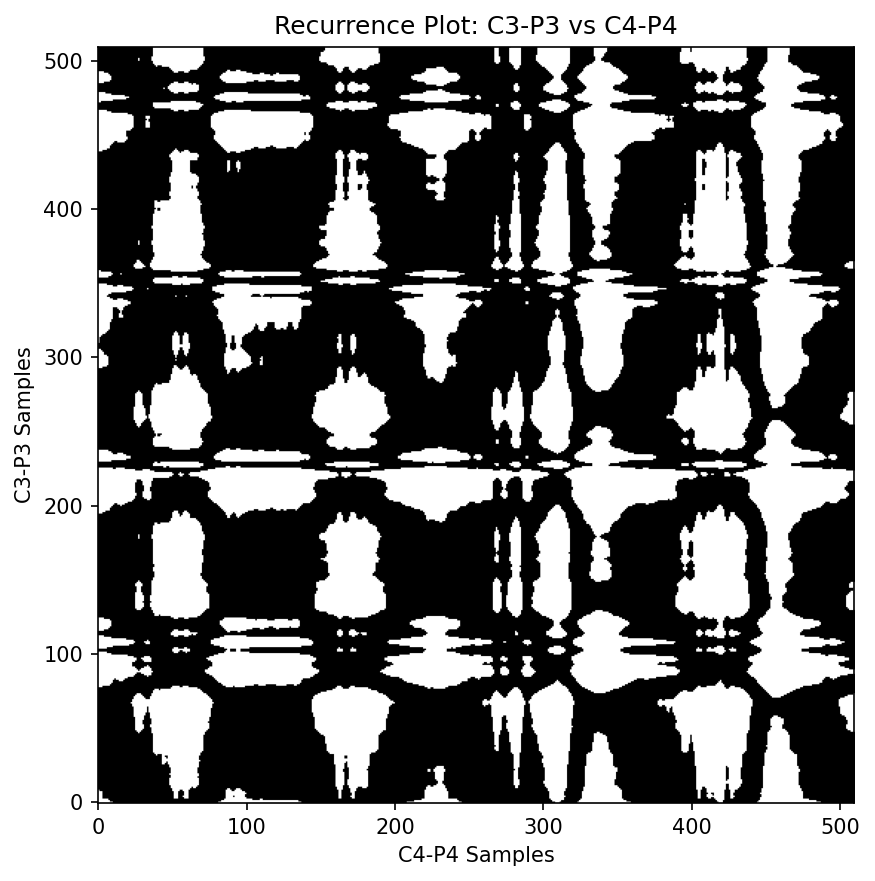
\includegraphics[width=\textwidth]{rr_compare/r03_epil.png}
					\caption{radius fraction = 0.2}
					\label{subfig:rp4}
				    \end{subfigure}

				    \caption{Cross recurrence plots for the selected EEG channel pairs, for an epileptic window. (a) R = 0.1 (b) R = 0.15 (c) R = 0.2 (d) R = 0.3}
				    \label{fig:rp_grid}
				\end{figure}


%				CRQA requires embedding the time series in a phase space to capture nonlinear dynamics. For each window pair from two channels, the optimal time delay (\(\tau\)) and embedding dimension (\(m\)) are determined as follows:

%				\begin{itemize}
%				    \item \textbf{Time Delay (\(\tau\))}: The Average Mutual Information (AMI) method is used to estimate \(\tau\), implemented via the \texttt{find\_optimal\_tau\_ami} function. AMI is computed for delays up to a maximum of 25 samples, and the first local minimum is selected as the optimal \(\tau\). The minimum \(\tau\) of the two channels is used to ensure compatibility.
%				    \item \textbf{Embedding Dimension (\(m\))}: The False Nearest Neighbors (FNN) method, implemented in the \texttt{false\_nearest\_neighbors} function, determines the optimal \(m\). Dimensions are tested up to a maximum of 10, with relative tolerance (\texttt{rtol}=15.0) and absolute tolerance (\texttt{atol}=2.0). The smallest dimension where the FNN ratio stabilizes is chosen, and the minimum \(m\) between the two channels is used.
%				\end{itemize}

				\subsection{Cross Recurrence Quantification Analysis (CRQA)}
				\label{subsec:crqa}

				CRQA quantifies the recurrent patterns between pairs of EEG channels within each time window. The \texttt{pyrqa} library is used with OpenCL acceleration for efficient computation. The process is as follows:

				\begin{enumerate}
				    \item \textbf{Time Series Length Validation}: For each window pair, the lenght's of the two time series are compared on having same length to ensure compatibility.
				    \item \textbf{Phase Space Reconstruction}: The time series are embedded into a phase space using the optimal \(\tau\) and \(m\), via the \texttt{TimeSeries} class in \texttt{pyrqa}.
				    \item \textbf{Radius Selection}: The radius for defining recurrence is computed using the Phase Space Separation (PSS) method (\texttt{pss} function). The maximum distances in the phase spaces of both channels are averaged to obtain a mean diameter, and the radius is set to 15\% of this value (\texttt{radius\_fraction=0.15}).
				    \item \textbf{CRQA Computation}: The \texttt{RQAComputation} class constructs a cross-recurrence matrix using a \texttt{FixedRadius} neighborhood, Euclidean metric, and Theiler corrector of 1. The computation yields 16 CRQA features, listed in Table~\ref{tab:pyrqa_metrics}, plus the segment label as the 17th feature.
				\end{enumerate}

				\begin{table}[h]
				\centering
				\caption{Quantitative measures computed by PyRQA}
				\label{tab:pyrqa_metrics}
				\begin{tabular}{ll}
				\toprule
				\textbf{Metric} & \textbf{Abbreviation} \\
				\midrule
				Recurrence Rate & RR \\
				Determinism & DET \\
				Average Diagonal Line Length & \(L_{\text{avg}}\) \\
				Longest Diagonal Line Length & \(L_{\text{max}}\) \\
				Divergence & DIV \\
				Entropy Diagonal Lines & \(H_{\text{diag}}\) \\
				Laminarity & LAM \\
				Trapping Time & TT \\
				Longest Vertical Line Length & \(V_{\text{max}}\) \\
				Average White Vertical Line Length & \(W_{\text{avg}}\) \\
				Longest White Vertical Line Length & \(W_{\text{max}}\) \\
				Longest White Vertical Line Divergence & \(W_{\text{max}}^{-1}\) \\
				Entropy Vertical Lines & \(H_{\text{vert}}\) \\
				Entropy White Vertical Lines & \(H_{\text{wvert}}\) \\
				Ratio of Determinism to Recurrence Rate & DET/RR \\
				Ratio of Laminarity to Determinism & LAM/DET \\
				\bottomrule
				\end{tabular}
				\end{table}


				\subsection{Algorithm Summary}
				\label{subsec:algorithm}

				The methodology is summarized in Algorithm~\ref{alg:crqa_computation}, which outlines the CRQA computation for each window and channel pair.

				\begin{algorithm}
				\caption{Cross Recurrence Quantification Analysis (CRQA) for EEG Windows}
				\label{alg:crqa_computation}
				\begin{algorithmic}[1]
				\State \textbf{Input}: EEG windows \( \{X_{c,w}\} \) for channels \( c \in C \), windows \( w = 1, \dots, N_w \), where \( N_w = \text{number of windows} \), number of electrodes \( N_e \)
				\State \textbf{Output}: CRQA feature matrix \( M \) of shape \( (N_w, N_e, N_e, 17) \)

				\For{each window index \( w = 1 \) to \( N_w \)}
				    \For{each channel pair \( (c_1, c_2) \in C \times C \)}
					\State \textbf{Time Series Preparation}
					\State Truncate time series \( X_{c_1,w} \) and \( X_{c_2,w} \) to minimum length
					\State \textbf{Set embedding parameters}
					\State Set \( \tau = 1 \)
					\State Set \( m = 3 \)
					\State \textbf{CRQA Computation}
					\State Construct cross-recurrence plot for \( (X_{c_1,w}, X_{c_2,w}) \) using \texttt{PyRQA} with:
					\State \quad Fixed radius neighborhood \( r = 0.15 \times \text{mean diameter} \), Euclidean metric, Theiler corrector = 1
					\State Extract 16 CRQA features: \{RR, DET, \( L_{\text{avg}} \), \( L_{\text{max}} \), DIV, \( H_{\text{diag}} \), LAM, TT, \( V_{\text{max}} \), \( W_{\text{avg}} \), \( W_{\text{max}} \), \( W_{\text{max}}^{-1} \), \( H_{\text{vert}} \), \( H_{\text{wvert}} \), DET/RR, LAM/DET\}
					\State \textbf{Feature Storage}
					\State Append window label \( l_w \) to features
					\State Store features in \( M[w, c_1, c_2, :] \)
				    \EndFor
				\EndFor

				\State \textbf{Return} RQA feature matrix \( M \)
				\end{algorithmic}
				\end{algorithm}

				 \subsection{Feature aggregation}
				 \label{subsec:feature_aggregation}
				 The resulting RQA feature matrix has dimensions \([N_w, N_e, N_e, 17]\), where \(N_w\) is the number of windows, 
				\(N_e\) is the number of channels, and 17 represents the 16 CRQA features plus the segment label(epileptic or normal). 
				 To summarize CRQA features across all channel pairs for each window, 
				 a mean feature matrix is computed by averaging the 16 CRQA features across all channel pairs, 
				 resulting in a final matrix of shape \([N_w, 17]\), where the last column retains the window label. 
				 This matrix summarizes the average dynamical interactions within each window.


				\subsection{Class Imbalance in RQA-EEG Data}

				Real world EEG datasets for epileptic seizure detection are by their nature imbalanced, 
				reflecting the transient nature of seizure's occurence in contrast to normal brain activity. 
				In our aggregated dataset, derived from CRQA features across the multi-channel EEG recordings,
				the distribution is stark: 98.29\% normal segments (19,926 examples) against 1.71\% epileptic (346 examples), 
				yielding a $\sim$58:1 ratio. This skew is a well known challenge in machine 
				learning which is often reffered as the "imbalanced learning problem".

				As discussed by He and Garcia\cite{he2009}, standard classifiers, (f.e, Random Forest), 
				can achieve misleadingly high accuracy ($\sim$99\%) 
				by over-predicting the majority class, resulting in poor recall for epileptic events.
				In RQA based models, this bias can minimize the effects of discriminative patterns, 
				such as the elevated determinism (DET) or laminarity (LAM) in epileptic signals with 
				false negatives posing ethical risks, delaying interventions, while naive oversampling 
				(f.e, duplication) incorporates the risk of overfitting in minority RQA features.

				In order to mitigate this, data-level resampling strategies can be employed, focusing on 
				synthetic generation to enrich the minority class without discarding information gained from
				the majority class. 

				\begin{table}[h]
				\centering
				\caption{Class distribution in the preprocessed RQA-EEG dataset, highlighting severe imbalance.}
				\label{tab:imbalance}
				\begin{tabular}{lcc}
				\toprule
				Class & Percentage (\%) & Count \\
				\midrule
				Normal (0) & 98.29 & 19,926 \\
				Epileptic (1) & 1.71 & 346 \\
				\bottomrule
				\end{tabular}
				\end{table}
				
				\subsection{Imbalance Mitigation: SMOTE Oversampling}

				Synthetic Minority Over-sampling Technique (SMOTE), 
				is a data level method that can generate synthetic epileptic samples
				by interpolating between minority instances and their k-nearest neighbors in 
				feature space \cite{SMOTEref}. Unlike random duplication, 
				SMOTE promotes diversity, reducing overfitting risks in low-sample regimes (e.g., our 346 epileptic examples). For RQA features---which capture non-linear dynamical patterns like recurrence rate (RR) and divergence (DIV)---this preserves subtle variations in epileptic trajectories without introducing artifacts.

				In implementation, SMOTE ($k=5$) is applied during training (post-stratified split) to balance the dataset to $\sim$50:50, yielding $\sim$19,000 synthetic samples. It integrates seamlessly with our Random Forest classifier via scikit-learn's imbalanced-learn library. Preliminary results show marked improvements: epileptic recall rises from 0.41 to 0.71, with macro F1 increasing to 0.81 (Table~\ref{tab:smote-impact}). This aligns with benchmarks in EEG seizure detection, where SMOTE enhances minority sensitivity by 20-30\% \cite{sharma2014smote}.

				Evaluation employs 5-fold stratified cross-validation and imbalance-aware metrics (F1-macro, precision-recall AUC), ensuring generalizability across RQA-derived datasets.
			\newpage


\bibliographystyle{plain}
\bibliography{references}

\end{document}
